\documentclass[xetex, unicode, 10pt, aspectratio=169]{beamer}
\usepackage{sty/style}
\usepackage{hyperref}
\usepackage{ragged2e}
\usepackage{xeCJK}
\usepackage[normalem]{ulem}
\usepackage{soul}
\usepackage{pdfpages}
\usepackage{setspace}
\usepackage{color, colortbl}
\usepackage{tikz}
% 自訂主題區

\xeCJKsetup{AutoFallBack = true}
% 啟用字型Fallback

\definecolor{backgroundcolor}{RGB}{240, 240, 240}
\definecolor{textcolor}{RGB}{0, 0, 0}
\definecolor{maincolor}{RGB}{89, 43, 31}
\definecolor{accentcolor}{RGB}{89, 43, 31}

\setCJKmainfont[
    BoldFont = IBMPlexSansTC-SmBld
]{IBMPlexSansTC-Text}
\setCJKfallbackfamilyfont{\CJKrmdefault}{PingFang SC}
\setsansfont[
    BoldFont = HelveticaNeue-Bold ,
    ItalicFont = HelveticaNeue-Italic ,
    BoldItalicFont = HelveticaNeue-BoldItalic ,
    ] {HelveticaNeue}
\setmonofont{Menlo-Regular}

% \setCJKmainfont[
%     BoldFont = IBMPlexSansTC-SmBld
% ]{IBMPlexSansTC-Text}
% \setCJKfallbackfamilyfont{\CJKrmdefault}{PingFang SC}
% \setsansfont[
%     BoldFont = SFProDisplay-Semibold ,
%     ItalicFont = SFProDisplay-RegularItalic ,
%     BoldItalicFont = SFProDisplay-BoldItalic ,
% ] {SFProDisplay-Regular}
% \setmonofont{SFMono-Regular}

% Tikz Settings for drawing commit graphs
\usetikzlibrary{shapes.geometric, arrows}
\tikzstyle{commit} = [rectangle, rounded corners, minimum
    width=0.6in, minimum height=0.2in, text centered, draw=black,
font=\footnotesize\ttfamily]
\tikzstyle{activecommit} = [commit, top color=green!15, bottom color=green!30]
\tikzstyle{greyedcommit} = [commit, top color=lightgray!30, bottom
color=lightgray!60]
\tikzstyle{arrow} = [thick,->,>=latex]

\title{Git 版控系統}
\subtitle{Git Version Control System}
\date{\today}
\author{Ostrichbeta Chan 陳逸銘}
\institute{WHUAI Team}

\begin{document}
\maketitle

\section{Git 簡介}

\begin{frame}{為什麼我們要學習版控系統?}
    若沒有版控系統,備份不同的版本,只能一個版本一個資料夾:
    \begin{center}
        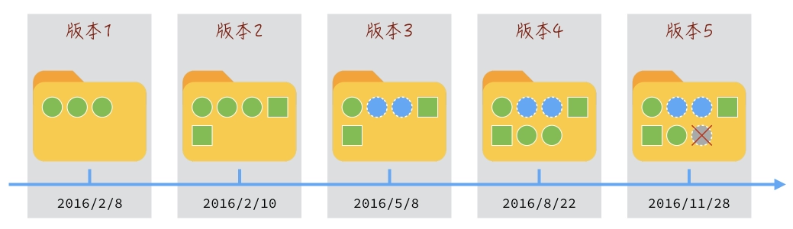
\includegraphics[width=3.75in]{./img/folders-without-vcs.png}
    \end{center}
    \begin{itemize}
        \item Chan 基於版本 5 開發了版本 6
        \item Lee 由版本 4 修復了一些 Bug 希望同步到最新開發中
        \item Yang 希望能夠快速的提煉出不同版本之間的區別給 Chang 老師彙報進度
    \end{itemize}
    \pause
    \begin{center}
        \Emph{沒有一個快速高效的方法,三個人都很頭大}
    \end{center}
\end{frame}

\begin{frame}{Git 的優點}
    開發管理 Linux 核心的 Linus Torvalds 在 2005
    年也遇到了這個問題,加之當時版控系統不盡完善(有的還死貴),於是他花了 10 天時間完成了 Git 的初版並開源,經過多年發展,Git 系統已經十分完善。
    \pause

    Git 有很多優點:

    \begin{itemize}
        \item \Emph{開放原始碼}\quad{}可以免費用,且有社群維護
        \item \Emph{快速高效}\quad{}Git 可以快速在不同版本間切換,特殊的設計使多版本下的目錄的空間佔用降低
        \item \Emph{分散式系統}\quad{}Git 不依賴伺服器,可以不受網路影響的使用
        \item \Emph{易上手}\quad{}雖然 Git 有眾多指令,但大概 20\% 的指令可以完成 80\% 的工作
    \end{itemize}
\end{frame}

\begin{frame}{Git 的安裝}
    \begin{itemize}
        \item Linux:使用各發行版的包管理器(apt, dnf, yum)直接安裝或由原始碼編譯後安裝
        \item macOS:安裝 Xcode Command Line Tools 過程中自動安裝
        \item Windows:由 Git 官網下載安裝檔安裝
    \end{itemize}

    Git 官方網站
    \underline{\href{https://git-scm.com/}{https://git-scm.com/}} 提供了
    Windows, macOS 和 Linux 的安裝檔
\end{frame}

\begin{frame}{預備知識}
    \begin{itemize}
        \item git 預設的編輯器是 \texttt{vim},可以瞭解 \texttt{vim} 的常用快速鍵,或使用
            \texttt{git config --global core.editor nano} 改用更友善的 \texttt{nano} 編輯器。
        \item Bash 中可以在輸入指令的過程中按 Tab 鍵自動補全
        \item Bash 中可使用上下方向鍵快速填入歷史指令
        \item Bash 和 Zsh 中用 Ctrl-A 跳至行頭,Ctrl-E 跳至行尾,Ctrl-C 終止當前程式,Ctrl-L 清除螢幕
        \item 在終端機中,可以使用 Shift-Ctrl-C 複製,Shift-Ctrl-V 貼上
        \item vim 的預設退出方法是按下 Esc 使 \texttt{-- INSERT --} 字樣消失,然後輸入 :q 退出
    \end{itemize}
\end{frame}

\begin{frame}{內容約定}
    \begin{itemize}
        \item 以下的 git 指令大多數在 git v2.39 版本下於 macOS 15.1 下執行
        \item 指令中出現尖括弧的部分如 \texttt{<text>} 為指令中必須填入的項
        \item 指令中出現方括弧的部分如 \texttt{[text]} 為指令中的可選項
        \item 除非特別說明,否則\Emph{所有的括弧符號都不需要輸入}
    \end{itemize}
\end{frame}

\section{Git 基本操作}

\subsection{Git 本機工作流程}

\begin{frame}{Git 的主要工作流程}
    \begin{center}
        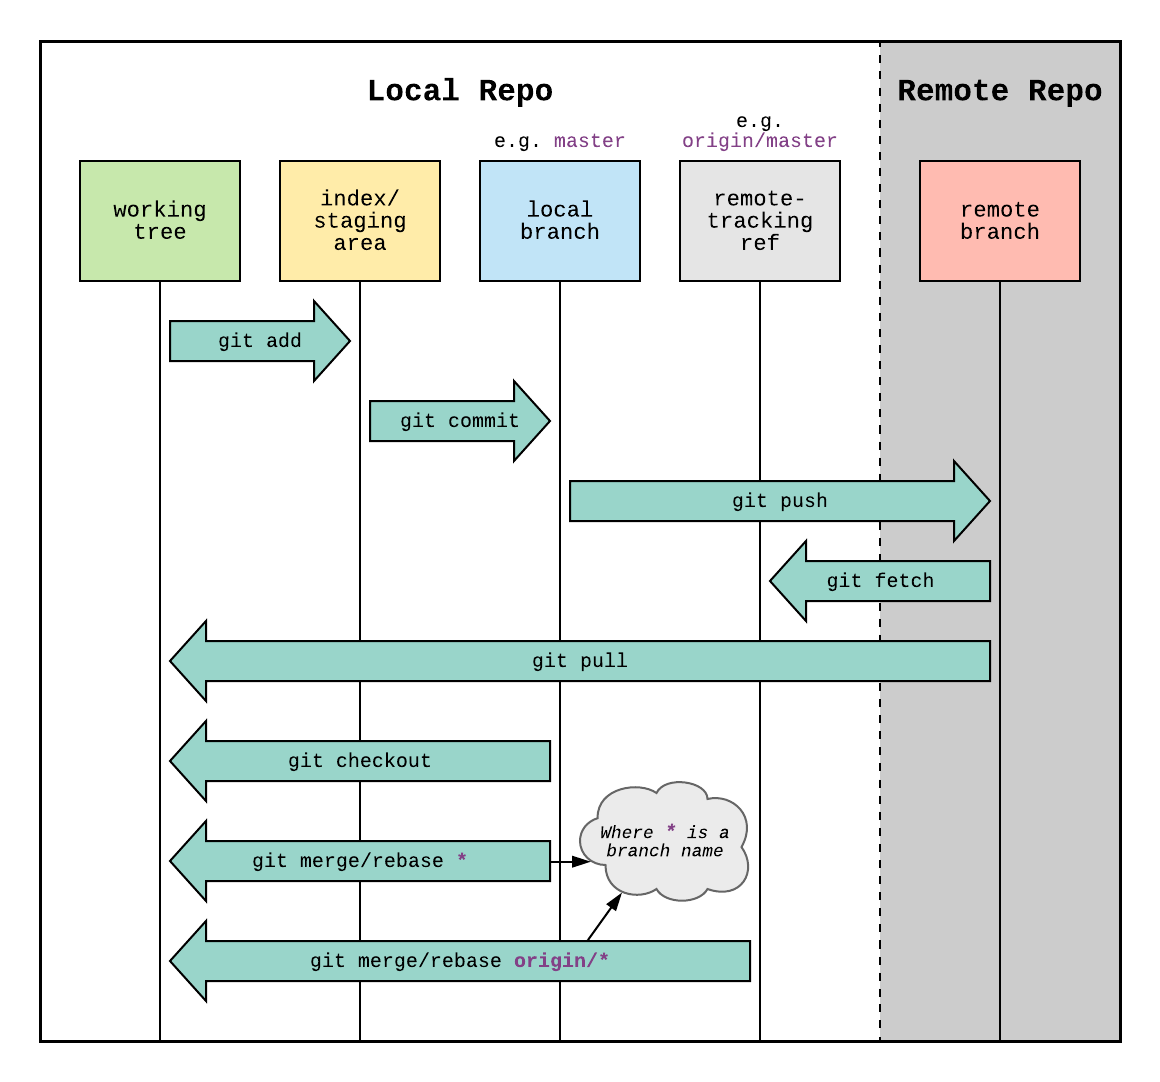
\includegraphics[height=2.5in]{./img/git-workflow.png}\\
        Git 流程簡圖
    \end{center}
\end{frame}

\begin{frame}{Git 的主要工作流程}
    \begin{columns}
        \begin{column}{0.6\textwidth}
            \begin{center}
                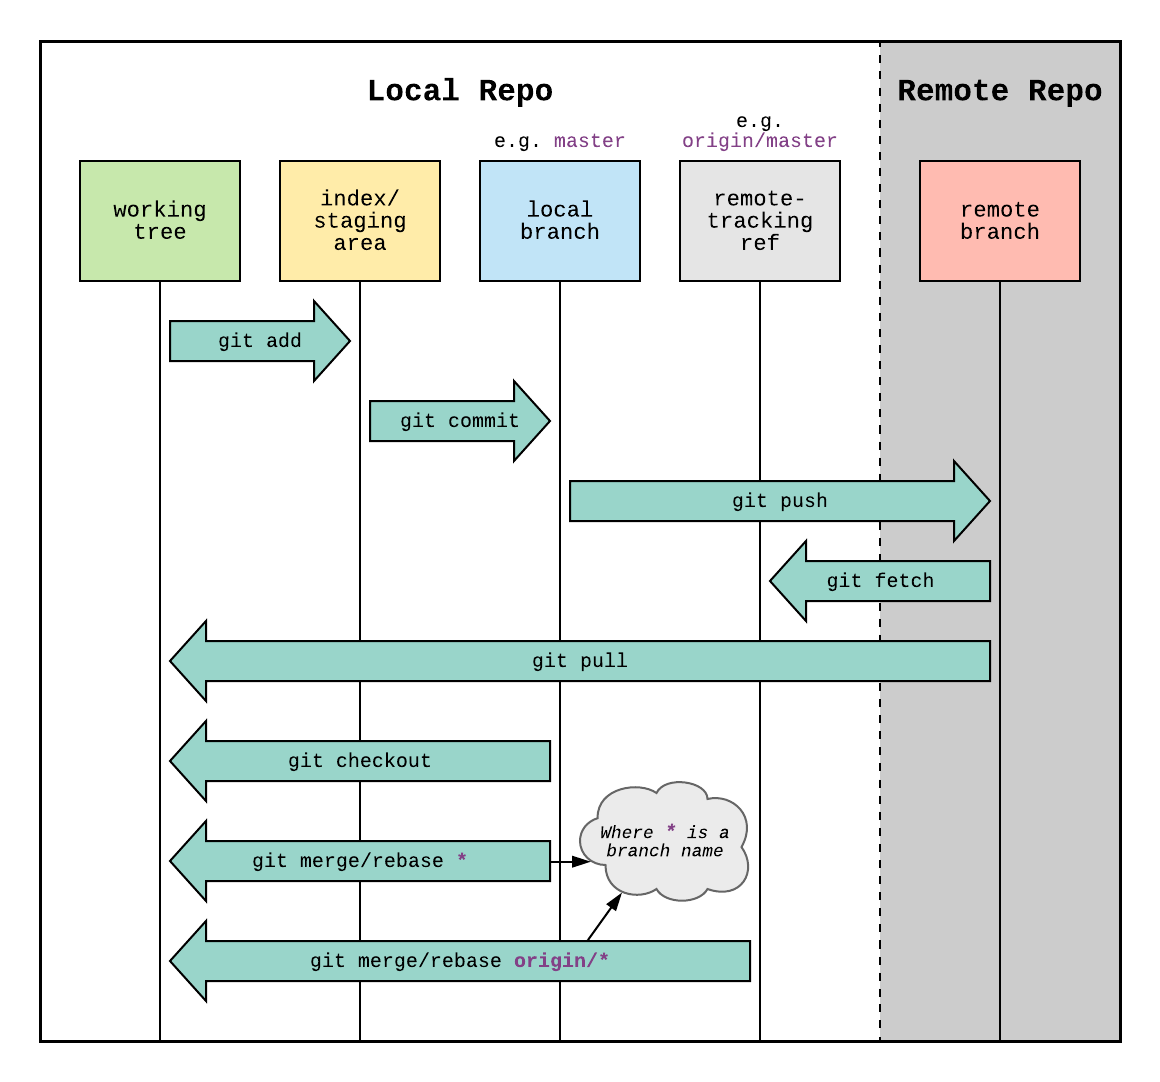
\includegraphics[height=2.7in]{./img/git-workflow.png}
            \end{center}
        \end{column}
        \begin{column}{0.4\textwidth}
            Git 的主要工作流程有以下部分:
            \pause
            \begin{itemize}
                \item 將文件加至 Git 版控
                \item 提交文件的變更
                \item 推送 commit 到遠端倉庫
                \item 取得遠端代碼變更
                \item 切換分支
                \item 合併不同分支\\
                    etc.
            \end{itemize}
        \end{column}
    \end{columns}
\end{frame}

\begin{frame}{Git 的主要工作流程}
    最簡單的 Git 流程:
    \begin{enumerate}
        \item 初始設定工作區
        \item 新增文件至版控系統
        \item 提交文件的修改
    \end{enumerate}

    如果需要與遠端倉庫溝通:
    \begin{enumerate}
            \setcounter{enumi}{3}
        \item 將修改推至雲端
    \end{enumerate}
\end{frame}

\subsection{環境設定}

\begin{frame}[fragile]{設定個人資訊}
    使用 Git 的第一件事是設定我們的個人資訊,方便 Git 記錄代碼的提交者。

    可以使用 \texttt{git config} 指令進行設定:
    \begin{lstlisting}[
            language = bash,
            numbers = left,
            linewidth = \textwidth
            ]
git config --global user.name <Name>
git config --global user.email <email>\end{lstlisting}

    執行後,可使用以下指令確認:
    \begin{lstlisting}[
        language = bash,
        numbers = left,
        linewidth = \textwidth
      ]
git config --global user.name
git config --global user.email\end{lstlisting}
\end{frame}

\begin{frame}{設定個人資訊}
    \begin{center}
        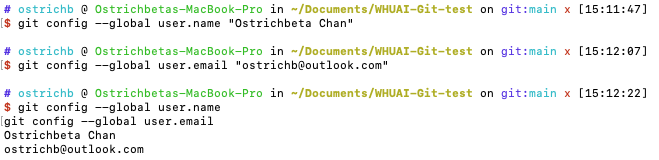
\includegraphics[height=1.3in]{./img/set-name-email.png}

        執行範例
    \end{center}
\end{frame}

\begin{frame}{設定個人資訊}
    使用 \texttt{git config --list} 還可以檢視當前 Git 的所有設定。
    \begin{center}
        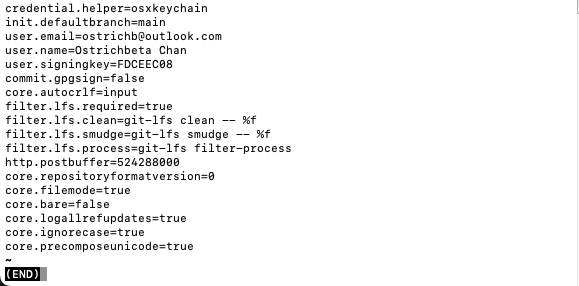
\includegraphics[height=2in]{./img/git-config-list.png}
    \end{center}
\end{frame}

\subsection{Git 主要指令}

\begin{frame}{本地工作常用指令}
    本章重點講解以下指令:
    \begin{columns}
        \begin{column}{0.3\textwidth}
            \begin{itemize}
                \item \texttt{git init}
                \item \texttt{git add}
                \item \texttt{git commit}
                \item \texttt{git reset}
                \item \texttt{git branch}
            \end{itemize}
        \end{column}

        \begin{column}{0.3\textwidth}
            \begin{itemize}
                \item \texttt{git checkout}
                \item \texttt{git merge}
                \item \texttt{git status}
                \item \texttt{git log}
            \end{itemize}
        \end{column}
    \end{columns}
\end{frame}

\begin{frame}{新增倉庫}
    \begin{block}{git init}
        在工作空間中使用 \texttt{git init} 可以將當前目錄交由 Git 接管。
    \end{block}
    \begin{center}
        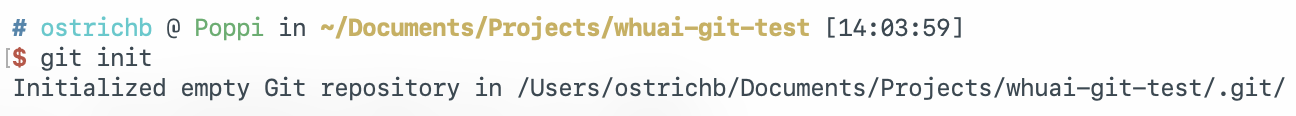
\includegraphics[width=5in]{./img/git-init.png}
    \end{center}
    \pause
    \begin{itemize}
        \item 一個 \texttt{.git} 目錄會被新增,此為 Git 的核心
        \item 移除這個 \texttt{.git} 目錄將會移除 Git 的控制\\
    \end{itemize}
    \Emph{整個專案⽬錄裡,什麼檔案或⽬錄刪了都救得回來,但  \texttt{.git} ⽬錄只要刪了就沒辦法了。}
\end{frame}

\begin{frame}{狀態查詢}
    \begin{block}{git status}
        取得當前工作空間的狀態,是否與遠端同步,檔案的提交狀態等。
        \begin{center}
            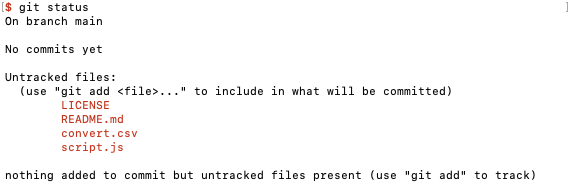
\includegraphics[width=5in]{./img/git-status-no-commit.png}\\
            當前有未管控的檔案
        \end{center}
    \end{block}
\end{frame}

\begin{frame}{狀態查詢}
    \begin{block}{git status}
        取得當前工作空間的狀態,是否與遠端同步,檔案的提交狀態等。
        \begin{center}
            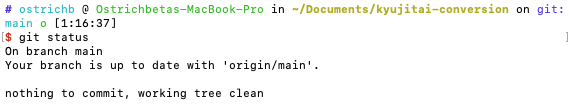
\includegraphics[width=5in]{./img/git-status-clean.png}\\
            已與遠端同步,且未有未提交的檔案
        \end{center}
    \end{block}
\end{frame}

\begin{frame}{往 Git 中新增檔案}
    \begin{block}{git add}
        將某些檔案/目錄加至 staging area (暫存區),為提交作準備。
        \begin{center}
            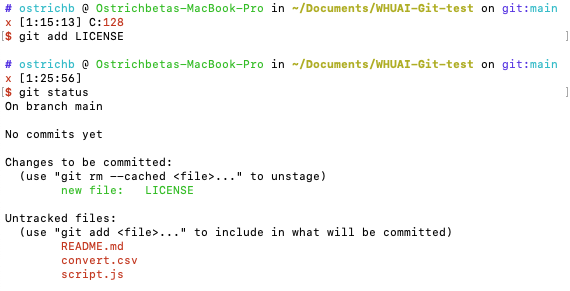
\includegraphics[width=4in]{./img/git-add-a-file.png}
        \end{center}
    \end{block}
\end{frame}

\begin{frame}{往 Git 中新增檔案}
    \begin{block}{git add}
        將某些檔案/目錄加至 staging area (暫存區),為提交作準備。
        \begin{itemize}
            \item 使用 \texttt{git add .} 可以將當前目錄所有檔案加至暫存區
            \item 若檔案有修改,需要再執行一次 \texttt{git add} 指令暫存變更
            \item 空目錄是無法提交的
            \item 使用 \texttt{git diff} 可詳細的查詢檔案具體的變更內容
        \end{itemize}
    \end{block}
    \pause
    \begin{block}{那要怎麼移除檔案?}
        \begin{itemize}
            \item 用 \texttt{rm} 移除檔案,然後 \texttt{git add} 追加變更至暫存區
            \item 或使用 \texttt{git rm} 指令完成上述兩步
        \end{itemize}
    \end{block}
\end{frame}

\begin{frame}[fragile]{往 Git 中提交檔案}
    \begin{block}{git commit}
        將暫存區中的檔案提交本地倉庫存檔。
        \begin{lstlisting}[
          language = bash,
          numbers = left,
          linewidth = \textwidth
        ]
git commit [-m <comment>]\end{lstlisting}
        \texttt{<comment>}為這一次提交的內容簡括,是代碼溝通的重要資訊,以下是一些良好的範例:
        \begin{lstlisting}[
          language = bash,
          numbers = left,
          linewidth = \textwidth
        ]
git commit -m "feat(auth): add JWT-based authentication"
git commit -m "fix(login): resolve race condition in login flow"\end{lstlisting}
        \dots 以及部分反面示範:
        \begin{lstlisting}[
          language = bash,
          numbers = left,
          linewidth = \textwidth
        ]
git commit -m "Update project"
git commit -m "Update readme and fix login issue"\end{lstlisting}
    \end{block}
\end{frame}

\begin{frame}[fragile]{往 Git 中提交檔案}
    \begin{block}{git commit}
        將暫存區中的檔案提交本地倉庫存檔。
        \begin{center}
            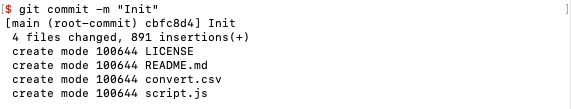
\includegraphics[width=4.5in]{./img/git-commit.png}
        \end{center}
        \begin{itemize}
            \item 未加入暫存區的檔案\textbf{將不會被提交}
            \item 提交內容信息是必須的,若不帶 \texttt{-m} 會彈出文字編輯器,需在其中加入文字
            \item 使用 \texttt{--amend} 不會新增 commit 而是追加到上一個 commit 中
        \end{itemize}
    \end{block}
\end{frame}

\begin{frame}{往 Git 中提交檔案}
    \begin{center}
        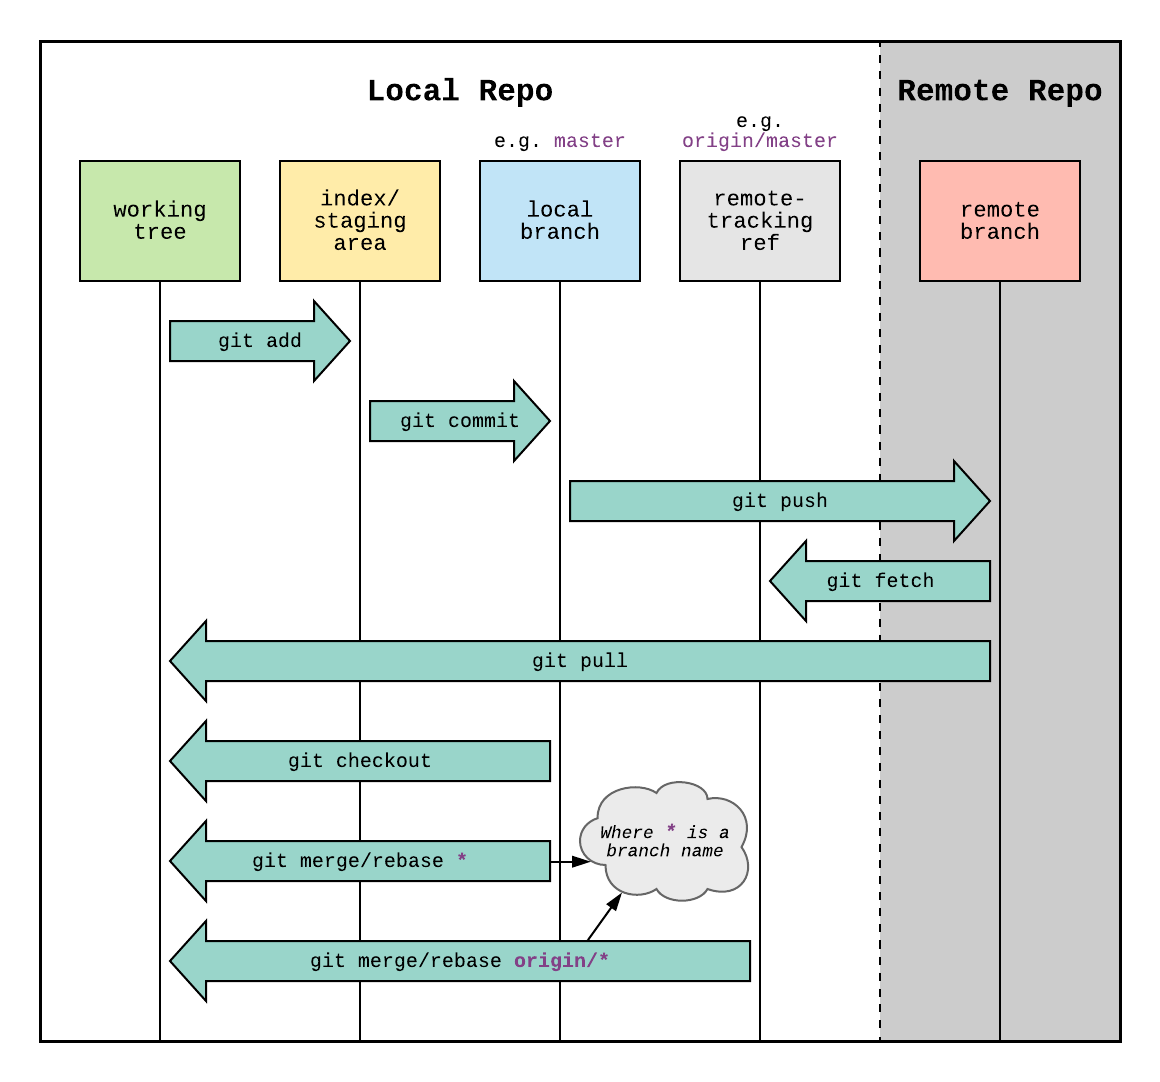
\includegraphics[height=2.7in]{./img/git-workflow.png}
    \end{center}
\end{frame}

\begin{frame}{Always remember to \texttt{git add} !}
    \begin{center}
        
\includegraphics[height=2.7in]{./img/always-remember-git-add.png}
    \end{center}
\end{frame}

\begin{frame}[fragile]{忽略部分檔案}
    \begin{block}{.gitignore}
        一些倉庫中會含有 .gitignore 檔, .gitignore 中記錄的檔案將不會被 Git 進行版本控制。

        倉庫中由編譯生成的檔案,或者是開發中所用的敏感存取密匙等通常都可加入 .gitignore 中。

        有以下幾種格式:

        \begin{lstlisting}[
          numbers = none,
          linewidth = \textwidth
        ]
/src/ # 忽略工作目錄下最上層的src目錄
src/ # 忽略所有名為src的目錄、子目錄
a.txt # 忽略所有名為 a.txt 的檔案
*.so # 忽略所有附檔名為 *.so 的檔案
!homo.so # 強制保留名為 homo.so 的檔案
/ros2/**/lah/ # ros2開頭 launch結尾的目錄/ros2/lah/和/ros2/s/s/lah/都符合\end{lstlisting}

        設定好之後將\ .gitignore 使用\ \texttt{git add} 新增,其規則就會對未來檔案生效。

        GitHub 官方也整理了一些環境和語言下常用的 .gitignore 檔案集:

        \underline{\href{https://github.com/github/gitignore}{https://github.com/github/gitignore}}
    \end{block}
\end{frame}

\begin{frame}[fragile]{忽略部分檔案}
    \begin{block}{.gitignore}
        .gitignore 設定的規則只對設定規則之後出現的檔案有效,已經存在但符合 .gitignore 規則的檔案仍然會被 Git 控制。

        如何將他們移出版控而不刪去檔案?
        \pause
        \begin{lstlisting}[
          language = bash,
          numbers = left,
          linewidth = \textwidth
        ]
git rm -r --cached . # 由版控中移除所有檔案
git add . # 新增所有檔案,但是將忽略 .gitignore 規則中的檔案
git commit -am "Remove ignored files"\end{lstlisting}

        具體可以參考

        \underline{\href{https://stackoverflow.com/questions/1274057/how-do-i-make-git-forget-about-a-file-that-was-tracked-but-is-now-in-gitignore}{\scriptsize
        https://stackoverflow.com/questions/1274057/how-do-i-make-git-forget-about-a-file-that-was-tracked-but-is-now-in-gitignore}}
    \end{block}

\end{frame}

\begin{frame}{檢視提交記錄}
    \begin{block}{git log}
        檢視過去的 commit 記錄,由新至舊排列。
        \begin{columns}
            \begin{column}{0.6\textwidth}
                \begin{center}
                    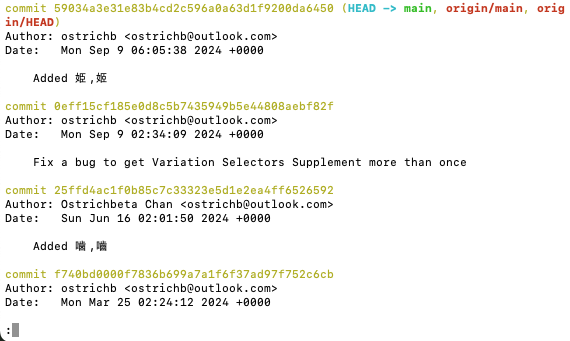
\includegraphics[width=3.2in]{./img/git-log.png}
                \end{center}
            \end{column}
            \begin{column}{0.4\textwidth}
                Log 預設會顯示:
                \begin{itemize}
                    \item 當前分支位置
                    \item commit 編號
                    \item commit 時間
                    \item commit 用戶
                \end{itemize}
            \end{column}
        \end{columns}
    \end{block}
\end{frame}

\begin{frame}{檢視提交記錄}
    \begin{block}{git log}
        檢視過去的 commit 記錄,由新至舊排列。

        \begin{itemize}
            \item 使用 \texttt{--oneline} 可以更緊湊的顯示記錄
            \item 使用 \texttt{--graph} 可以加入分支線顯示
        \end{itemize}
        \begin{columns}
            \begin{column}{0.5\textwidth}
                \begin{center}
                    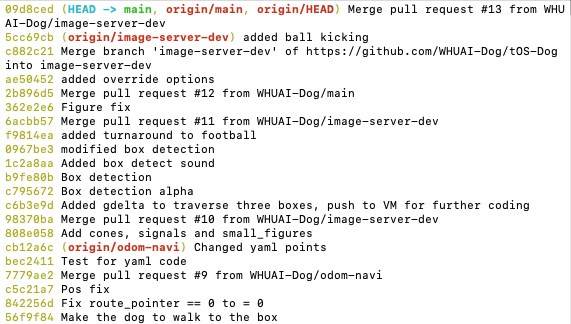
\includegraphics[width=2.5in]{./img/git-log-oneline.png}
                \end{center}
            \end{column}
            \begin{column}{0.5\textwidth}
                \begin{center}
                    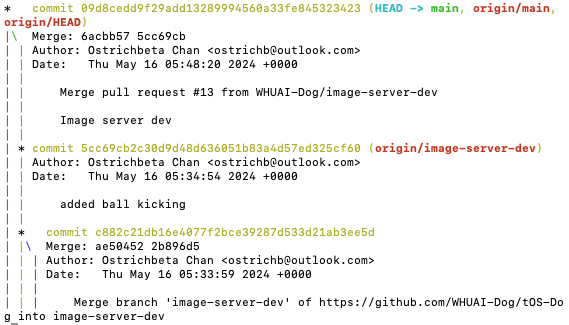
\includegraphics[width=2.5in]{./img/git-log-graph.png}
                \end{center}
            \end{column}
        \end{columns}
    \end{block}
\end{frame}

\begin{frame}[fragile]{退回更新}
    \begin{block}{git reset}
        可以將工作空間或目錄復原到之前某一次提交時的狀態。
        \begin{lstlisting}[
          language = bash,
          numbers = left,
          linewidth = \textwidth
        ]
git reset 0967be3 # Commit 號
git reset 0967be3^
git reset HEAD~2
git reset main~4\end{lstlisting}
        \pause
        \begin{itemize}
            \item 每⼀個 \^{} 符號表⽰前⼀次,\textasciitilde 表示前 n 次。如
                \texttt{HEAD\textasciitilde 2}表示 HEAD 的前兩次。
            \item \texttt{HEAD} 表示當前所在的分支狀態,而 \texttt{main} 則指向
                \texttt{main} 分支的最新狀態。
        \end{itemize}
    \end{block}
\end{frame}

\begin{frame}[fragile]{退回更新}
    \begin{block}{git reset}
        \texttt{git reset} 主要有三種工作模式。
        \begin{lstlisting}[
          language = bash,
          numbers = left,
          linewidth = \textwidth
        ]
git reset --mixed 0967be3 #若不帶參數,預設就是mixed
git reset --soft 0967be3
git reset --hard 0967be3\end{lstlisting}
        \pause
        \begin{itemize}
            \item Mixed 是預設的工作模式,不改變工作目錄,但將檔案退回到未追蹤的狀態;
            \item Soft 不改變工作目錄,將檔案退回到暫存區;
            \item Hard 改變工作目錄和暫存區,將檔案復原到目標分支的狀態(硬復原)。
        \end{itemize}
    \end{block}
\end{frame}

\begin{frame}{退回更新 - \texttt{git reset --mixed}}
    \begin{itemize}
        \item Mixed 是預設的工作模式,不改變工作目錄,但將檔案退回到未追蹤的狀態;
    \end{itemize}
    \begin{center}
        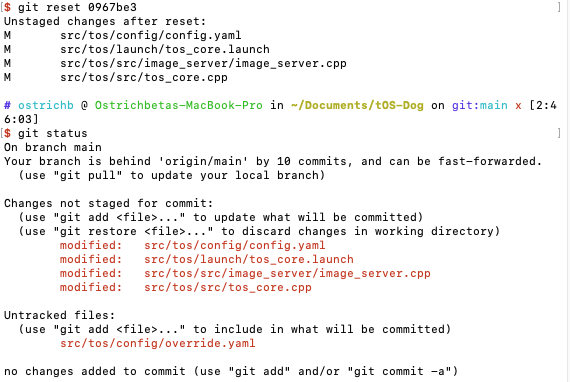
\includegraphics[width=3.0in]{./img/git-reset-mixed.png}
    \end{center}
\end{frame}

\begin{frame}{退回更新 - \texttt{git reset --soft}}
    \begin{itemize}
        \item Soft 不改變工作目錄,將檔案退回到暫存區;
    \end{itemize}
    \begin{center}
        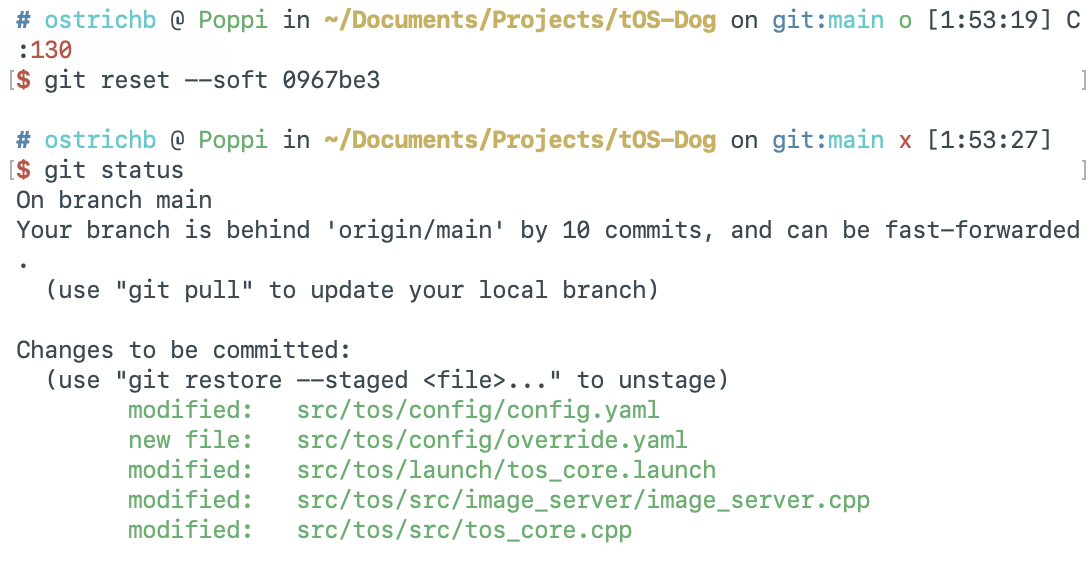
\includegraphics[width=3.3in]{./img/git-reset-soft.png}
    \end{center}
\end{frame}

\begin{frame}{退回更新 - \texttt{git reset --hard}}
    \begin{itemize}
        \item Hard 改變工作目錄和暫存區,將檔案復原到目標分支的狀態(硬復原)。
    \end{itemize}
    \begin{center}
        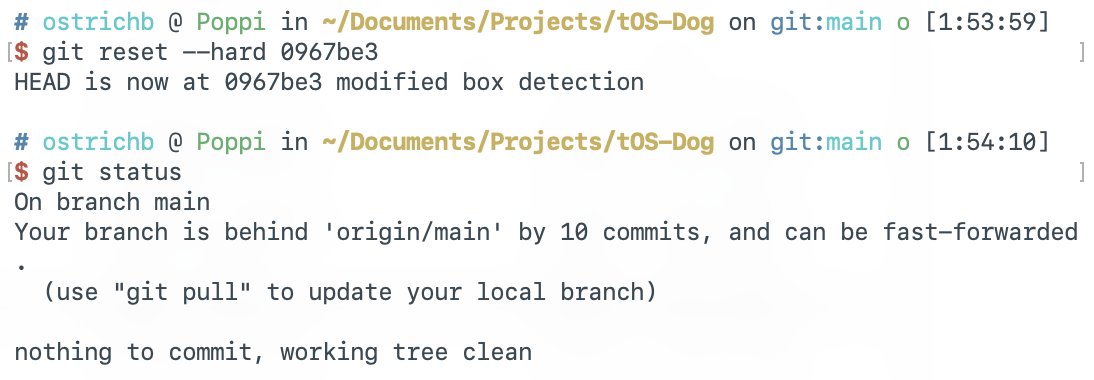
\includegraphics[width=3.3in]{./img/git-reset-hard.png}
    \end{center}
\end{frame}

\begin{frame}{退回更新}
    Hard 復原之後,還可以回到沒有執行 reset 之前的狀態嗎?
    \pause

    \emph{可以!}
    \begin{itemize}
        \item 使用 \texttt{git reflog} 指令找出所需要的分支
        \item 使用 \texttt{git reset --hard <commit>} 復原到目標分支
    \end{itemize}

    \begin{center}
        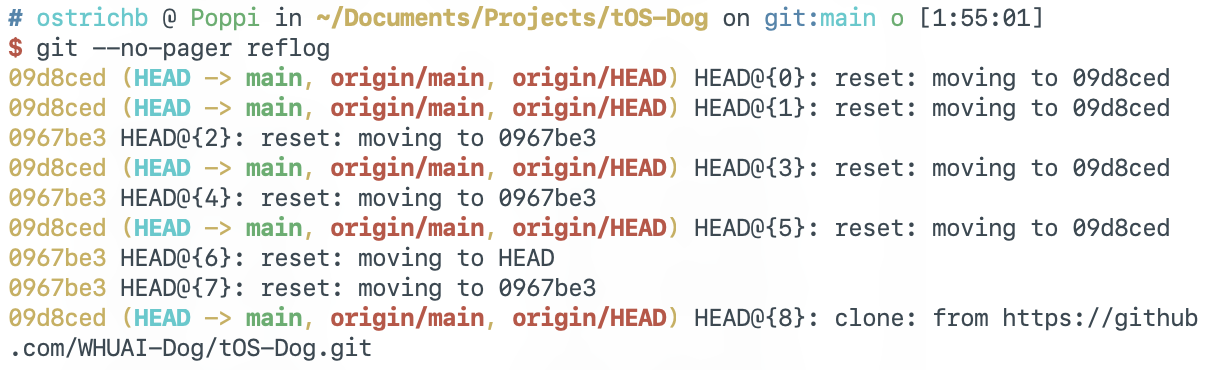
\includegraphics[width=3.5in]{./img/git-reflog.png}
    \end{center}
\end{frame}

\begin{frame}{Commit 的更新流程}
    一開始的時候假設有三個 commit:
    \begin{center}
        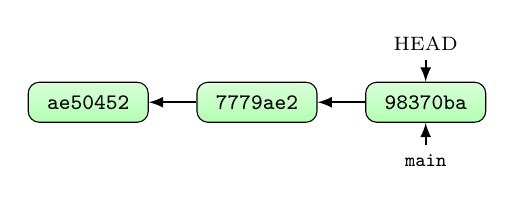
\begin{tikzpicture}
            % Commits
            \node[activecommit] (ae50452) {ae50452};
            \node[activecommit, right of=ae50452, xshift=0.45in] (7779ae2) {7779ae2};
            \node[activecommit, right of=7779ae2, xshift=0.45in] (98370ba) {98370ba};
            \node[draw=none, above of=98370ba, font=\scriptsize,
            yshift=-0.1in] (head) {HEAD};
            \node[draw=none, below of=98370ba, font=\scriptsize,
            yshift=+0.1in] (main) {\texttt{main}};
            % Arrows
            \draw[arrow] (7779ae2) -- (ae50452);
            \draw[arrow] (98370ba) -- (7779ae2);
            \draw[arrow] (head) -- (98370ba);
            \draw[arrow] (main) -- (98370ba);
        \end{tikzpicture}
    \end{center}
    \pause
    然後不小心錯誤的提交了一個不希望的 commit:
    \begin{center}
        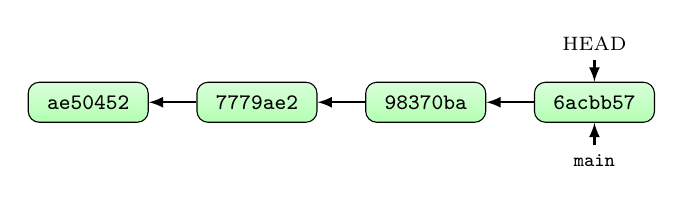
\begin{tikzpicture}
            % Commits
            \node[activecommit] (ae50452) {ae50452};
            \node[activecommit, right of=ae50452, xshift=0.45in] (7779ae2) {7779ae2};
            \node[activecommit, right of=7779ae2, xshift=0.45in] (98370ba) {98370ba};
            \node[activecommit, right of=98370ba, xshift=0.45in] (6acbb57) {6acbb57};
            \node[draw=none, above of=6acbb57, font=\scriptsize,
            yshift=-0.1in] (head) {HEAD};
            \node[draw=none, below of=6acbb57, font=\scriptsize,
            yshift=+0.1in] (main) {\texttt{main}};
            % Arrows
            \draw[arrow] (7779ae2) -- (ae50452);
            \draw[arrow] (98370ba) -- (7779ae2);
            \draw[arrow] (6acbb57) -- (98370ba);
            \draw[arrow] (head) -- (6acbb57);
            \draw[arrow] (main) -- (6acbb57);
        \end{tikzpicture}
    \end{center}
\end{frame}

\begin{frame}{Commit 的更新流程}
    然後不小心錯誤的提交了一個不希望的 commit:
    \begin{center}
        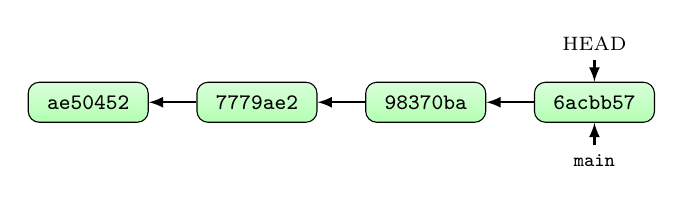
\begin{tikzpicture}
            % Commits
            \node[activecommit] (ae50452) {ae50452};
            \node[activecommit, right of=ae50452, xshift=0.45in] (7779ae2) {7779ae2};
            \node[activecommit, right of=7779ae2, xshift=0.45in] (98370ba) {98370ba};
            \node[activecommit, right of=98370ba, xshift=0.45in] (6acbb57) {6acbb57};
            \node[draw=none, above of=6acbb57, font=\scriptsize,
            yshift=-0.1in] (head) {HEAD};
            \node[draw=none, below of=6acbb57, font=\scriptsize,
            yshift=+0.1in] (main) {\texttt{main}};
            % Arrows
            \draw[arrow] (7779ae2) -- (ae50452);
            \draw[arrow] (98370ba) -- (7779ae2);
            \draw[arrow] (6acbb57) -- (98370ba);
            \draw[arrow] (head) -- (6acbb57);
            \draw[arrow] (main) -- (6acbb57);
        \end{tikzpicture}
    \end{center}
    \pause
    此時執行一次\texttt{git reset --hard}:
    \begin{center}
        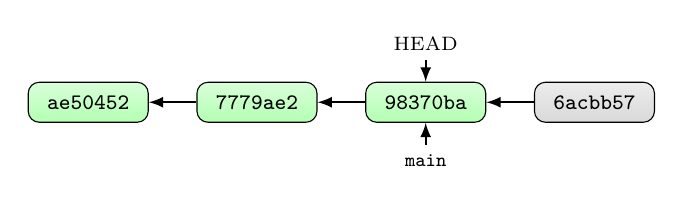
\begin{tikzpicture}
            % Commits
            \node[activecommit] (ae50452) {ae50452};
            \node[activecommit, right of=ae50452, xshift=0.45in] (7779ae2) {7779ae2};
            \node[activecommit, right of=7779ae2, xshift=0.45in] (98370ba) {98370ba};
            \node[greyedcommit, right of=98370ba, xshift=0.45in] (6acbb57) {6acbb57};
            \node[draw=none, above of=98370ba, font=\scriptsize,
            yshift=-0.1in] (head) {HEAD};
            \node[draw=none, below of=98370ba, font=\scriptsize,
            yshift=+0.1in] (main) {\texttt{main}};
            % Arrows
            \draw[arrow] (7779ae2) -- (ae50452);
            \draw[arrow] (98370ba) -- (7779ae2);
            \draw[arrow] (6acbb57) -- (98370ba);
            \draw[arrow] (head) -- (98370ba);
            \draw[arrow] (main) -- (98370ba);
        \end{tikzpicture}
        \pause

        \texttt{git reset --hard}僅僅是跳至了已經儲存在過去 \slash\ 未來的某個「狀態」,所以可以快速復原
    \end{center}
\end{frame}

\begin{frame}{分支}
    \begin{center}
        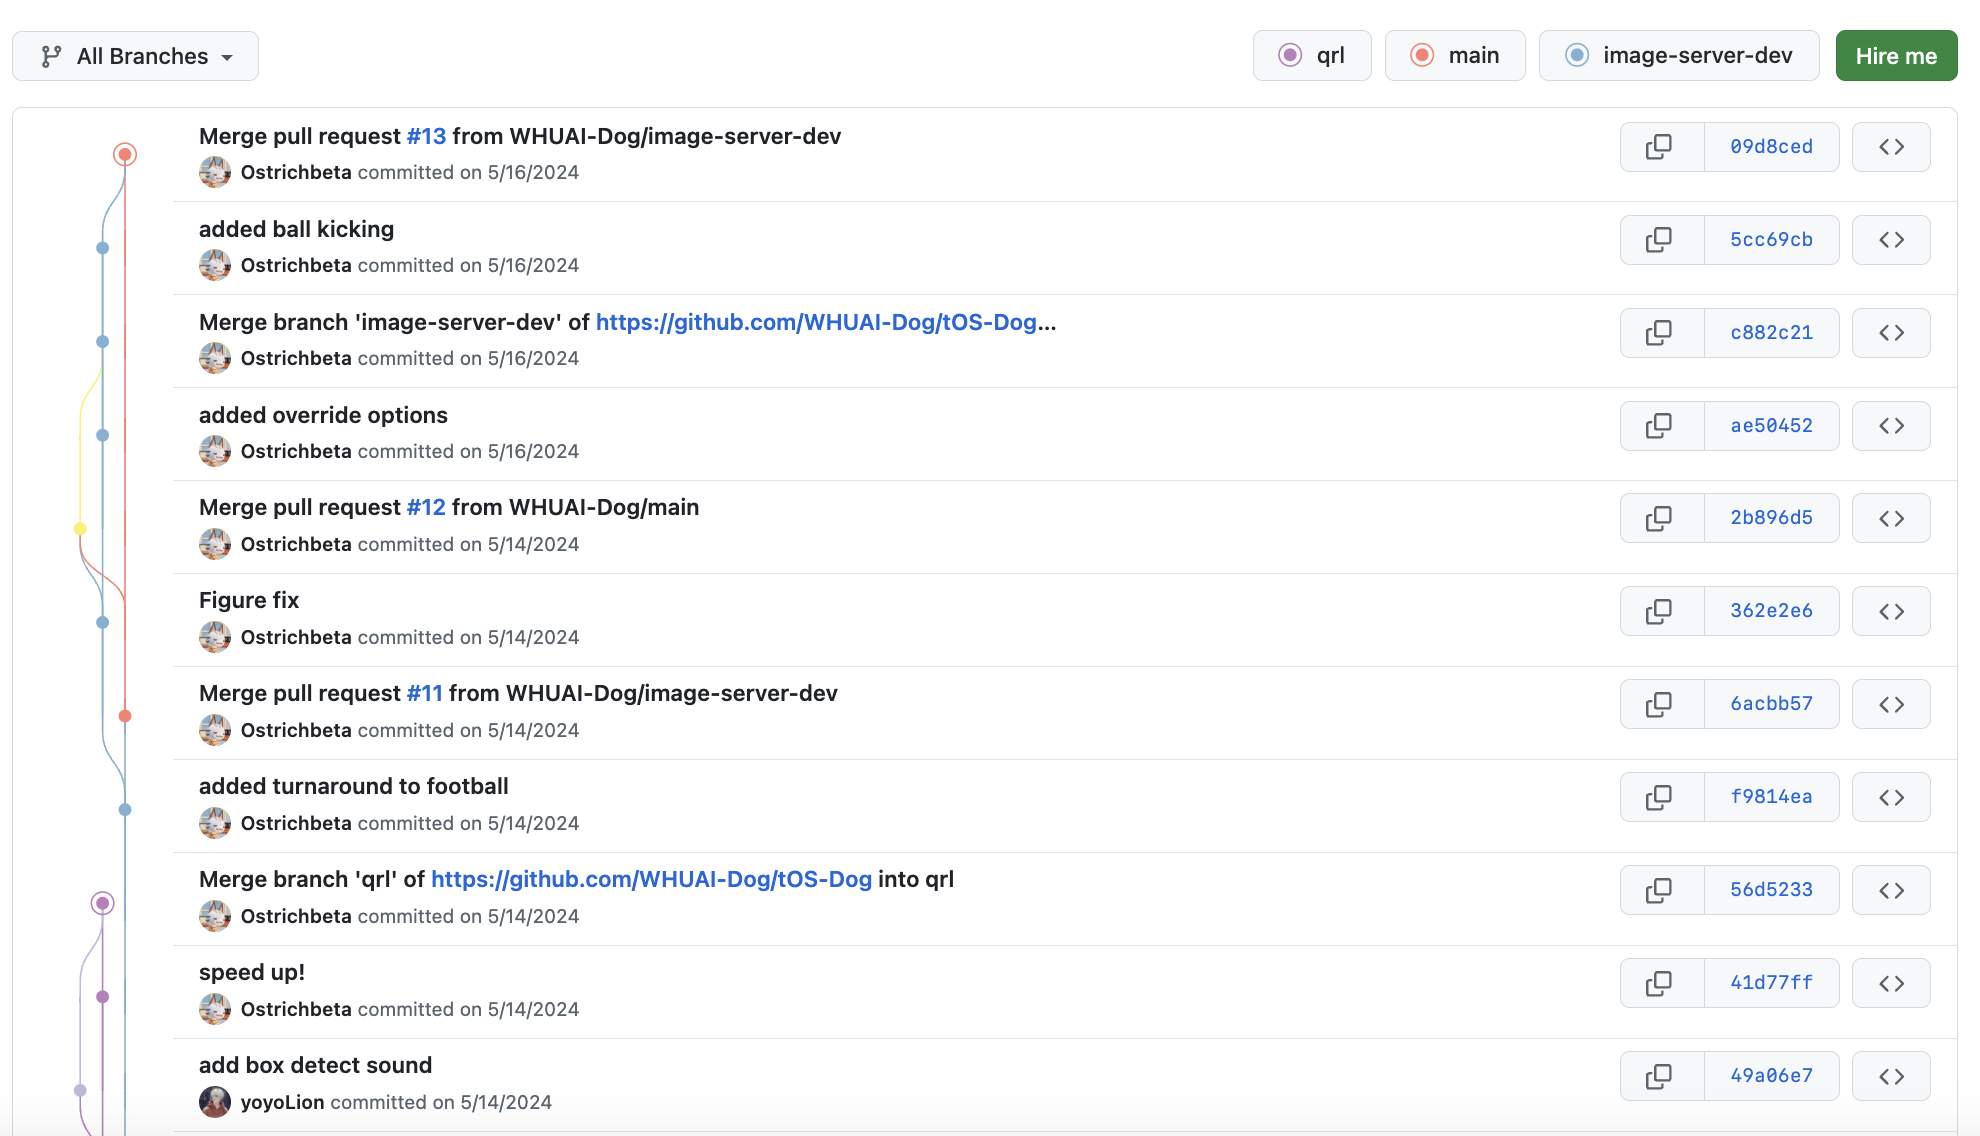
\includegraphics[width=4.2in]{./img/branches.png}\\
        多分支開發範例
    \end{center}
\end{frame}

\begin{frame}{分支}
    \begin{spacing}{1.75}
        \justifying\hspace{17pt} 在開發的過程中,⼀路往前 Commit
        也沒什麼問題,但當開始越來越多同伴⼀起在同⼀個專案⼯作的時候,可能就不能這麼隨興的想 Commit 就
        Commit,這時候分⽀就很好⽤。例如想要\Emph{增加新功能},或是\Emph{修正
        Bug},或是想\Emph{實驗看看某些新的做法},都可以另外做⼀個分⽀來進⾏,待做完確認沒問題之後再合併回來,不會影響正在運⾏的產品線。

        \justifying \hspace{17pt} 分支還可以方便的合併,就算不同分支之間可能存在衝突,Git 也會給出解決衝突的方法。

        \begin{center}
            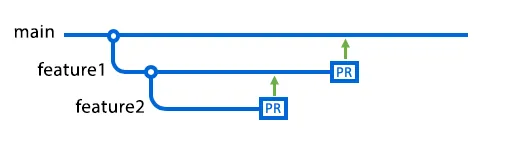
\includegraphics[width=3.5in]{./img/github-branches.png}
        \end{center}
    \end{spacing}
\end{frame}

\begin{frame}{管理分支}
    \begin{block}{git branch}
        \begin{itemize}
            \item \texttt{git branch}:檢視當前本機存在的分支
            \item \texttt{git branch -a}:檢視本機和遠端所有的分支(僅遠端可用\texttt{-r})
        \end{itemize}

        \begin{center}
            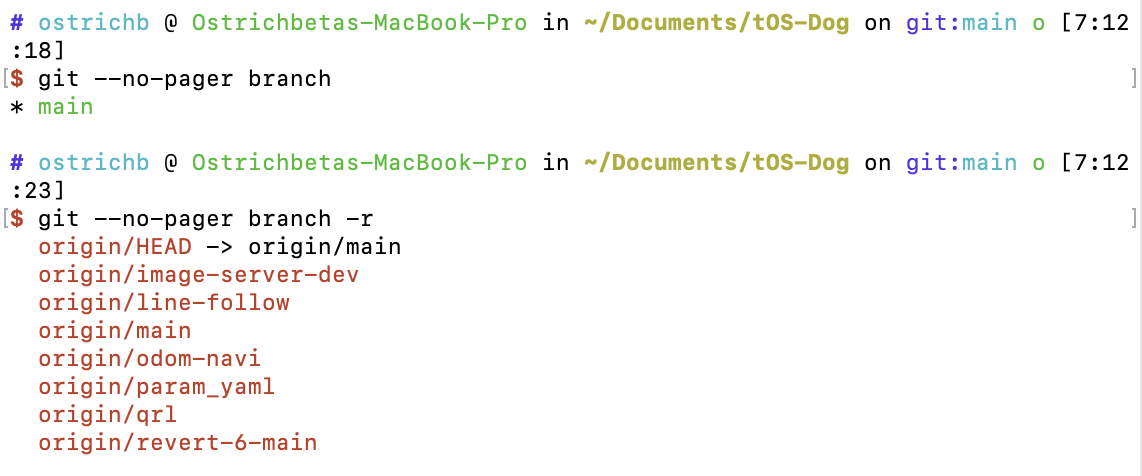
\includegraphics[width=4in]{./img/git-branch.png}\\
            \texttt{--no-pager} 直接輸出而不開啟文字編輯器
        \end{center}
    \end{block}

\end{frame}

\begin{frame}{管理分支}
    \begin{block}{git branch}
        \begin{itemize}
            \item \texttt{git branch -m <old> <new>}:將 \texttt{<old>}
                分支改名為 \texttt{<new>} 分支
            \item \texttt{git branch <branch>}:新增分支 \texttt{<branch>}
            \item \texttt{git branch -d <branch>}:移除分支 \texttt{<branch>}
        \end{itemize}

        \begin{center}
            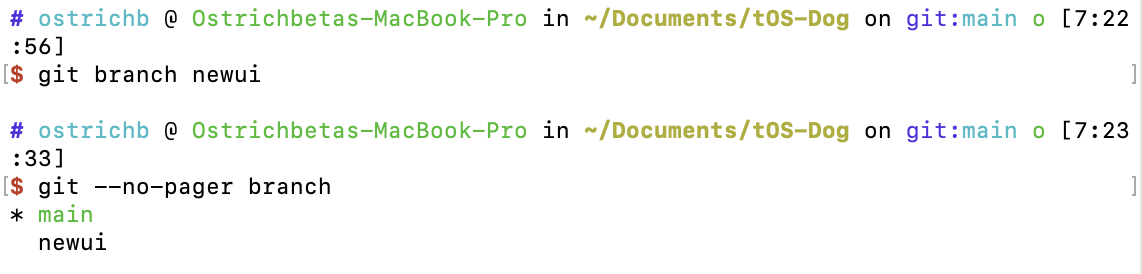
\includegraphics[width=4in]{./img/git-branch-create.png}
        \end{center}
    \end{block}
\end{frame}

\begin{frame}{分支切換}
    \begin{block}{git checkout}
        \begin{itemize}
            \item \texttt{git checkout <branch>}:跳到 \texttt{<branch>} 分支
            \item \texttt{git checkout -b <branch>}:跳到 \texttt{<branch>}
                分支,若分支不存在則新增
        \end{itemize}

        \begin{center}
            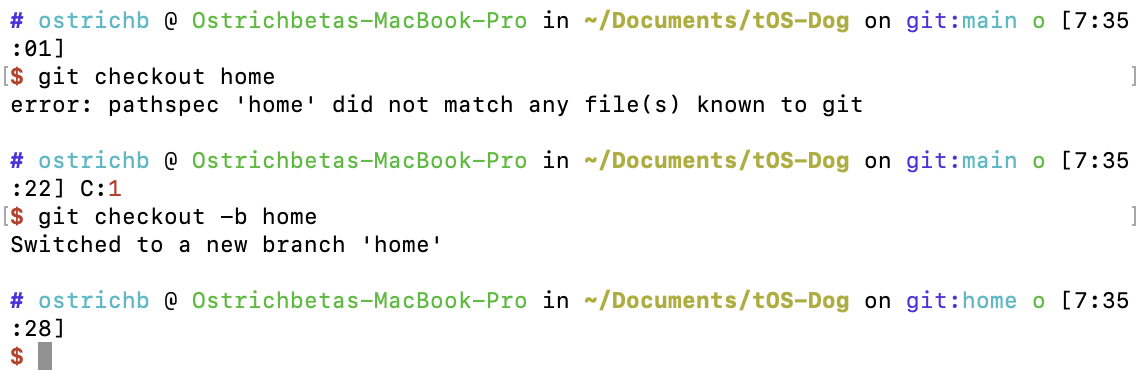
\includegraphics[width=4in]{./img/git-checkout.png}
        \end{center}
    \end{block}
\end{frame}

\begin{frame}{分支切換}
    \begin{center}
        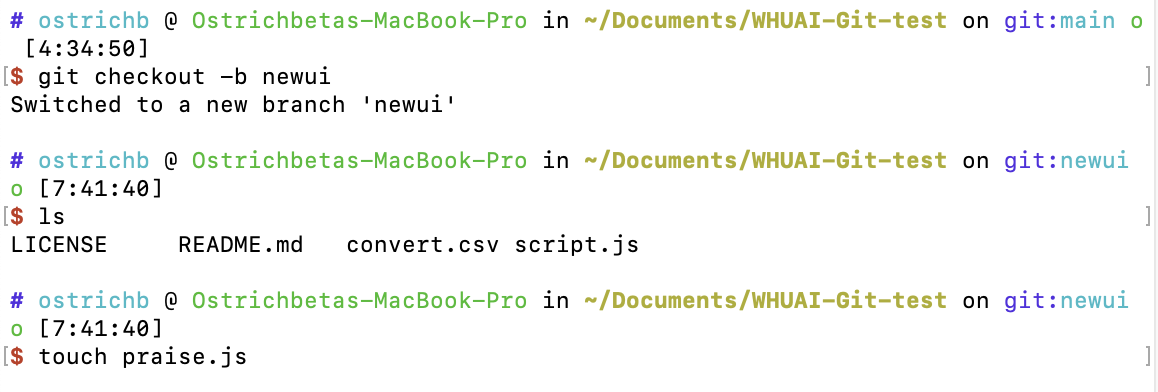
\includegraphics[width=4in]{./img/git-new-branch-0.png}
        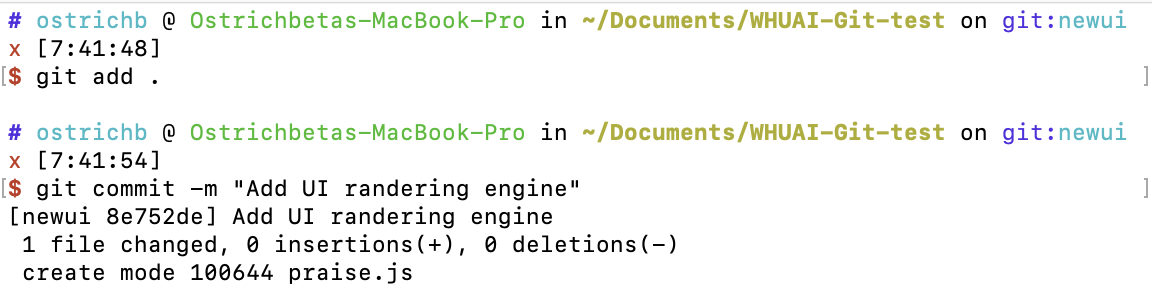
\includegraphics[width=4in]{./img/git-new-branch-1.png}
    \end{center}
\end{frame}

\begin{frame}{分支切換}
    \begin{center}
        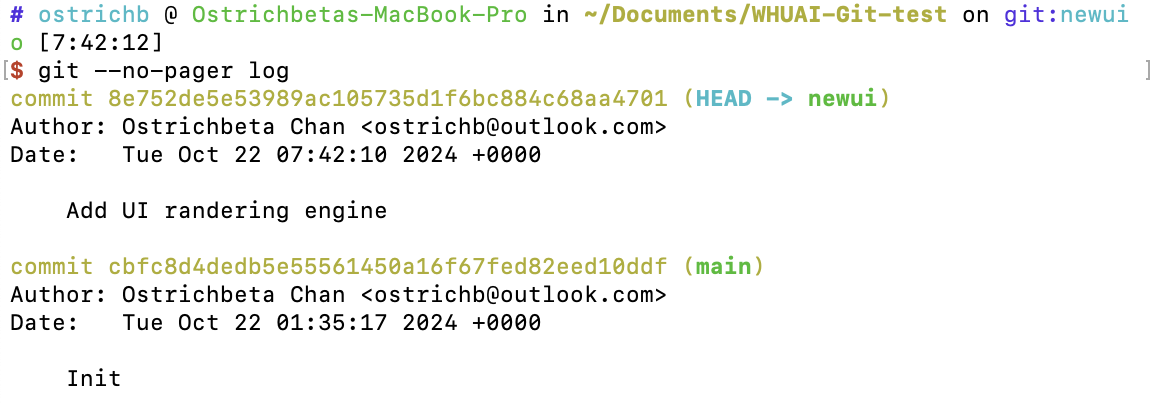
\includegraphics[width=4in]{./img/git-new-branch-2.png}

        Commit 之後原分支沒有改動,\texttt{HEAD} 指向當前的 \texttt{newui} 分支
    \end{center}
\end{frame}

\begin{frame}{分支合併}
    \begin{block}{git merge}
        \begin{itemize}
            \item \texttt{git merge [-m <comment>] <branch>}:將
                \texttt{<branch>} 分支\Emph{往當前分支合併}
        \end{itemize}

        \begin{center}
            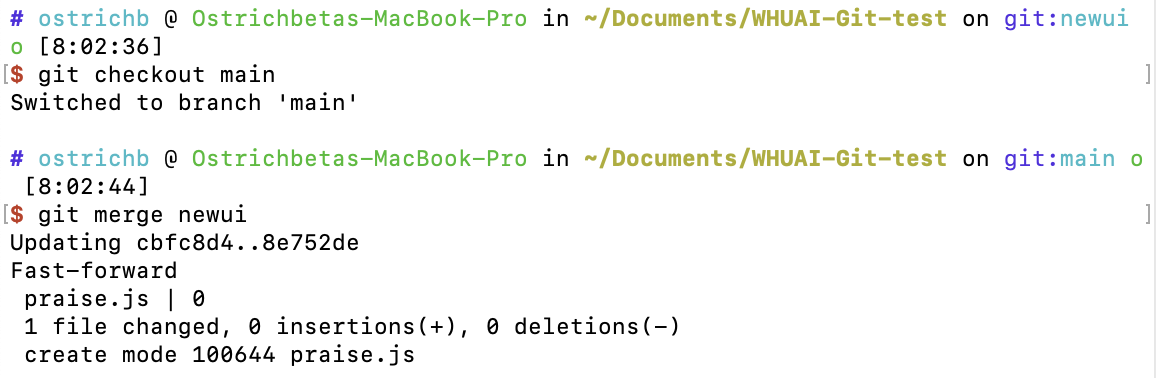
\includegraphics[width=4in]{./img/git-merge.png}

            由於分出 \texttt{newui} 後 \texttt{main} 沒有新的 commit,合併時可以直接快轉(fast-forward)
        \end{center}
    \end{block}
\end{frame}

\begin{frame}{分支合併}
    \begin{block}{git merge}
        \begin{center}
            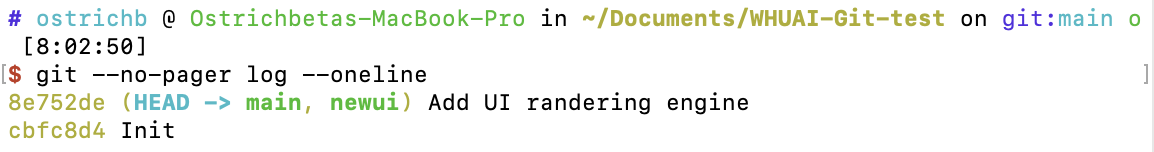
\includegraphics[width=4in]{./img/git-merge-log.png}

            合併後 \texttt{HEAD}, \texttt{main} 和 \texttt{newui} 都指向同一個 commit
        \end{center}
    \end{block}
\end{frame}

\begin{frame}[fragile]{分支合併}
    \begin{block}{無衝突的合併}
        一開始 \texttt{newui} 由 \texttt{main} 分支分出去,然後在 \texttt{newui} 中新增兩個檔案:
        \begin{lstlisting}[
          language = bash,
          numbers = none,
          linewidth = \textwidth
        ]
git checkout newui
touch auth.js
touch ui.html
git add .
git commit -m "Created UI file"\end{lstlisting}
        \texttt{main} 中 新增一個檔案:
        \begin{lstlisting}[
          language = bash,
          numbers = none,
          linewidth = \textwidth
        ]
git checkout main
touch api.js
git add .
git commit -m "Included API entrypoint"\end{lstlisting}
    \end{block}
\end{frame}

\begin{frame}{分支合併}
    現在分支樹長得像這樣:
    \begin{center}
        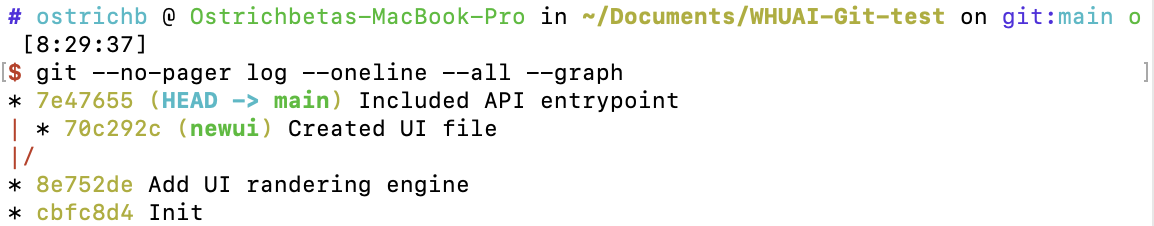
\includegraphics[width=4in]{./img/git-log-all-branches.png}
    \end{center}
    由於兩邊互不衝突也可以直接合併:
    \begin{center}
        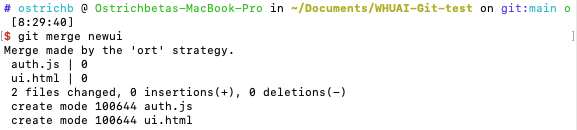
\includegraphics[width=4in]{./img/git-merge-no-conflict.png}
    \end{center}
\end{frame}

\begin{frame}{分支合併}
    \begin{block}{此時的 \texttt{newui} 是什麼狀態?}
        由於只是由 \texttt{newui} 併入 \texttt{main} 分支, \texttt{main} 分支包含了
        \texttt{newui} 分支的更動(即 auth.js 和 ui.html)。

        但是 \texttt{newui} 分支不會包含 \texttt{main} 在分出 \texttt{newui}
        後的那一部分改變(即沒有 api.js)。

        若要將 \texttt{HEAD}, \texttt{main} 和 \texttt{newui} 指向同一個
        commit,可以切到 \text{newui} 後 merge \texttt{main} 分支。
    \end{block}
\end{frame}

\begin{frame}{分支合併}
    \begin{center}
        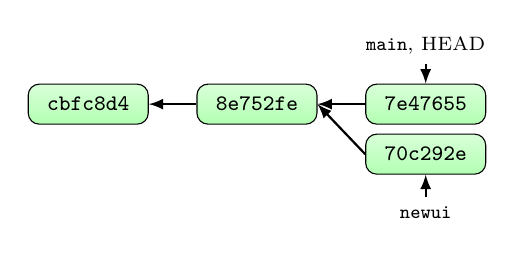
\begin{tikzpicture}
            % Commits
            \node[activecommit] (cbf) {cbfc8d4};
            \node[activecommit, right of=cbf, xshift=0.45in] (8e7) {8e752fe};
            \node[activecommit, right of=8e7, xshift=0.45in] (7e4) {7e47655};
            \node[activecommit, right of=8e7, xshift=0.45in,
            yshift=-0.25in] (70c) {70c292e};
            \node[draw=none, above of=7e4, yshift=-0.1in, font=\scriptsize]
            (main) {\texttt{main}, HEAD};
            \node[draw=none, below of=70c, yshift=+0.1in, font=\scriptsize]
            (newui) {\texttt{newui}};
            % Arrows
            \draw[arrow] (8e7) -- (cbf);
            \draw[arrow] (7e4) -- (8e7);
            \draw[arrow] (70c.west) -- (8e7.east);
            \draw[arrow] (main) -- (7e4);
            \draw[arrow] (newui) -- (70c);

        \end{tikzpicture}

        合併之前,兩個分支指向各自分隔的 commit

    \end{center}
\end{frame}

\begin{frame}{分支合併}
    \begin{center}
        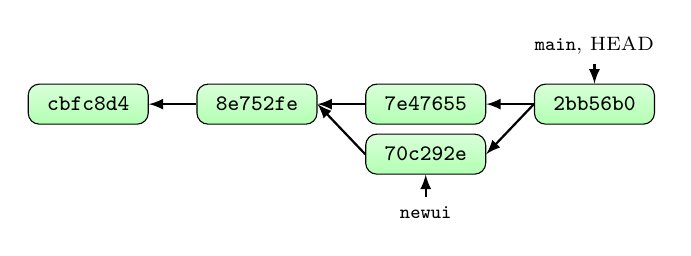
\begin{tikzpicture}
            % Commits
            \node[activecommit] (cbf) {cbfc8d4};
            \node[activecommit, right of=cbf, xshift=0.45in] (8e7) {8e752fe};
            \node[activecommit, right of=8e7, xshift=0.45in] (7e4) {7e47655};
            \node[activecommit, right of=8e7, xshift=0.45in,
            yshift=-0.25in] (70c) {70c292e};
            \node[activecommit, right of=7e4, xshift=0.45in] (2bb) {2bb56b0};
            \node[draw=none, above of=2bb, yshift=-0.1in, font=\scriptsize]
            (main) {\texttt{main}, HEAD};
            \node[draw=none, below of=70c, yshift=+0.1in, font=\scriptsize]
            (newui) {\texttt{newui}};
            % Arrows
            \draw[arrow] (8e7) -- (cbf);
            \draw[arrow] (7e4) -- (8e7);
            \draw[arrow] (70c.west) -- (8e7.east);
            \draw[arrow] (main) -- (2bb);
            \draw[arrow] (newui) -- (70c);
            \draw[arrow] (2bb) -- (7e4);
            \draw[arrow] (2bb.west) -- (70c.east);

        \end{tikzpicture}

        合併之後,\texttt{main} 指向合併後的 commit,但 \texttt{newui} 仍然指向原來合併之前的 commit

        \pause
        分支本質上\Emph{只是指向一個 commit 的指標}
    \end{center}
\end{frame}

\begin{frame}[fragile]{分支合併}
    \begin{block}{有衝突合併}
        假設 \texttt{main} 分支下有一檔案 EULA.txt:
        \begin{lstlisting}[
          language = bash,
          numbers = none,
          linewidth = \textwidth
        ]
This software is licensed.
Created by:\end{lstlisting}
        此時分出分支 EULA,更改了其內容並 commit 如下:
        \begin{lstlisting}[
          language = bash,
          numbers = none,
          linewidth = \textwidth
        ]
This software is licensed.
Created by:
Jeder Chan\end{lstlisting}
    \end{block}
\end{frame}

\begin{frame}[fragile]{分支合併}
    \begin{block}{有衝突合併}

        同時 \texttt{main} 分支中也更改了其內容:
        \begin{lstlisting}[
          language = bash,
          numbers = none,
          linewidth = \textwidth
        ]
This software is licensed.
Oreated by:
Ostrichbeta Chan\end{lstlisting}
        嘗試進行合併,會提示自動合併失敗,發生了\Emph{內容衝突}:
        \begin{center}
            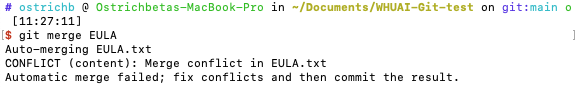
\includegraphics[width=4in]{./img/git-merge-failed.png}
        \end{center}
    \end{block}
\end{frame}

\begin{frame}[fragile]{分支合併}
    \begin{block}{有衝突合併}
        此時開啟 EULA.txt,可以看到 Git 標記出了衝突處。
        \begin{center}
            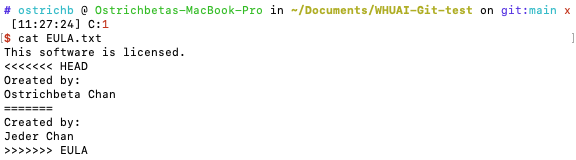
\includegraphics[width=3in]{./img/open-conflict-file.png}
        \end{center}
        \pause
        將其手動修改為不衝突的版本並去除所有標記:
        \begin{center}
            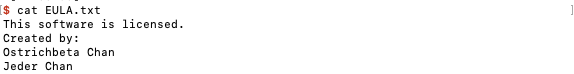
\includegraphics[width=3in]{./img/resolve-conflict.png}
        \end{center}
        然後再 \texttt{git add}, \texttt{git commit / git merge --continue} 即可解決衝突。
    \end{block}
\end{frame}

\begin{frame}{分支合併}
    \begin{block}{有衝突合併}
        Commit 後可以看到衝突已經解決,合併成功:
        \begin{center}
            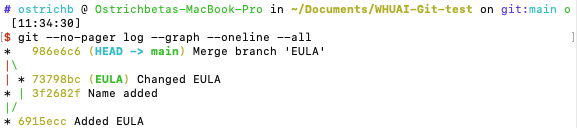
\includegraphics[width=4in]{./img/git-log-after-conflict-solved.png}
        \end{center}
    \end{block}
\end{frame}

\begin{frame}{分支合併}
    \begin{block}{有衝突合併}
        若主分支對檔案進行了改動,待合併分支將這個檔案刪除,此時合併會發生\Emph{修改/刪除衝突}:
        \begin{center}
            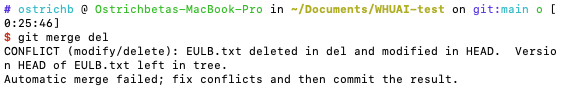
\includegraphics[width=4in]{./img/git-merge-modify-delete-conflict.png}
        \end{center}
        \pause

        有兩種解決方式:
        \begin{itemize}
            \item 使用 \texttt{git add <file>} 保留檔案,接受主分支的修改
            \item 使用 \texttt{git rm <file>} 刪去檔案,接受待合併分支的提交
        \end{itemize}

        解決衝突後使用 \texttt{git commit} 或 \texttt{git merge --continue} 繼續合併過程
    \end{block}
\end{frame}

\begin{frame}{分支合併}
    \begin{block}{有衝突合併}
        若主分支與待合併分支在合併時有一個內容不一樣的\Emph{同名非文字檔},稱為\Emph{新增/新增衝突}:

        \begin{center}
            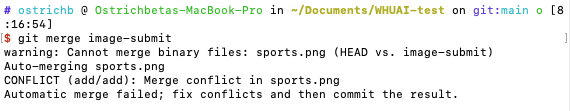
\includegraphics[width=4in]{./img/git-merge-add-add-conflict.png}
        \end{center}
        \pause

        有兩種解決方式:
        \begin{itemize}
            \item 使用 \texttt{git checkout --ours <file>} 使用主分支版本
            \item 使用 \texttt{git checkout --theirs <file>} 使用待合併分支版本
        \end{itemize}

        解決衝突後使用 \texttt{git commit} 或 \texttt{git merge --continue} 繼續合併過程

    \end{block}
\end{frame}

\begin{frame}{分支合併}
    \begin{block}{放棄合併}
        使用 \texttt{git merge --abort} 將會放棄當前的合併,將分支回到合併前狀態。
    \end{block}
\end{frame}

\subsection{其他指令}

\begin{frame}[fragile]{其他指令}
    \begin{block}{git rebase}
        將另外一個分支作為基準合併。
        \begin{lstlisting}[
          language = bash,
          numbers = none,
          linewidth = \textwidth
        ]
git rebase <branch>\end{lstlisting}
        其與 \texttt{git merge} 的區別如下圖所示。
        \begin{center}
            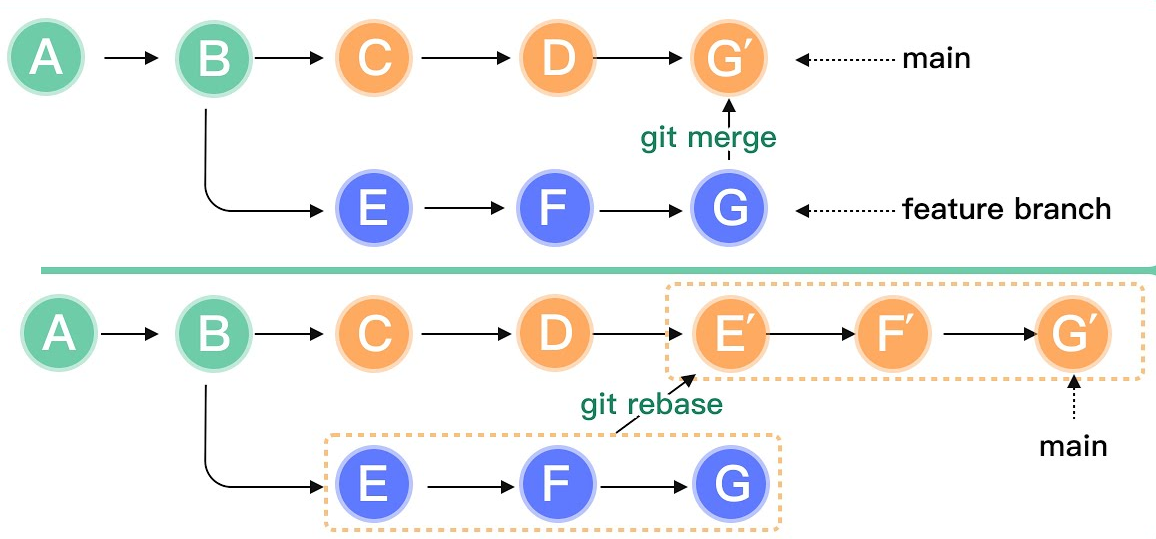
\includegraphics[width=2.8in]{./img/git-merge-vs-git-rebase.png}
        \end{center}
    \end{block}
\end{frame}

\begin{frame}[fragile]{其他指令}
    \begin{block}{git stash}
        暫存已經進入暫存區但尚未 commit 的檔案。
        \begin{lstlisting}[
          language = bash,
          numbers = none,
          linewidth = \textwidth
        ]
git stash # 暫存當前改動
git stash list # 列出當前的stash列表
git stash apply stash@{<id>} # 套用ID為 <id> 的 stash到當前分支上
git stash drop stash@{<id>} # 刪去一個 stash
git stash pop stash@{<id>} # 等同 apply + drop\end{lstlisting}

        使用 \texttt{git stash} 可以暫存所有「已被 git 追蹤已經放入或未有放入暫存區(staging area)」的變動,但不會暫存新增未被 git 管控或被忽略的檔案。
    \end{block}
\end{frame}

\begin{frame}[fragile]{其他指令}
    \begin{block}{git cherry-pick}
        抽出一個 commit 並整合到當前的 \texttt{HEAD}
        \begin{lstlisting}[
          language = bash,
          numbers = none,
          linewidth = \textwidth
        ]
git cherry-pick <commit> # 揀一個分支整合
git cherry-pick <commit1>...<commit2>
# 揀 commit1 至 commit2 之間的整合(不含 commit1)
git cherry-pick <commit1>^..<commit2>
# 揀 commit1 至 commit2 之間的整合(含 commit1)\end{lstlisting}
        \pause
        整合之後,新的 commit 改變的內容會與舊 commit 一致,但會有一個新的 commit 號。
        \begin{center}
            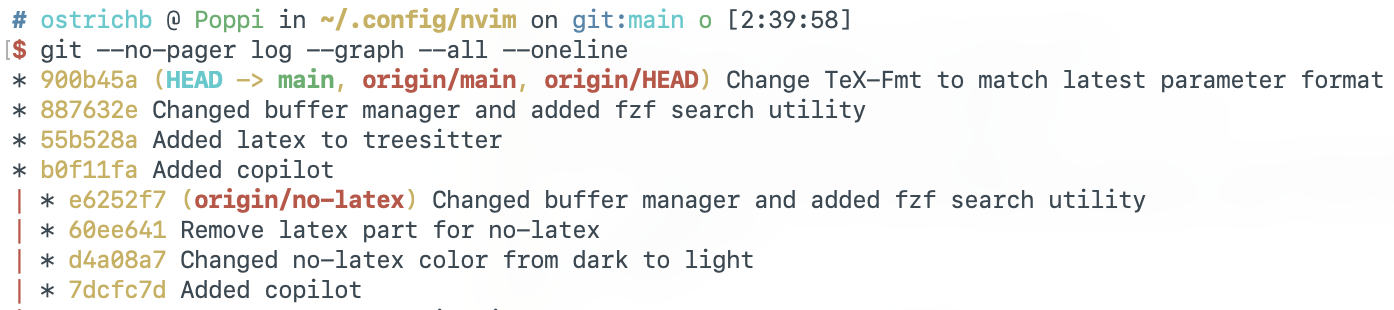
\includegraphics[width=4in]{./img/git-log-cherrypick.png}
        \end{center}
    \end{block}
\end{frame}

\begin{frame}[fragile]{其他指令}
    \begin{block}{git blame}
        檢視一個檔案中哪一行是由誰什麼時候在哪個 commit 中新增。
        \begin{lstlisting}[
          language = bash,
          numbers = none,
          linewidth = \textwidth
        ]
git blame <path>\end{lstlisting}

        \begin{center}
            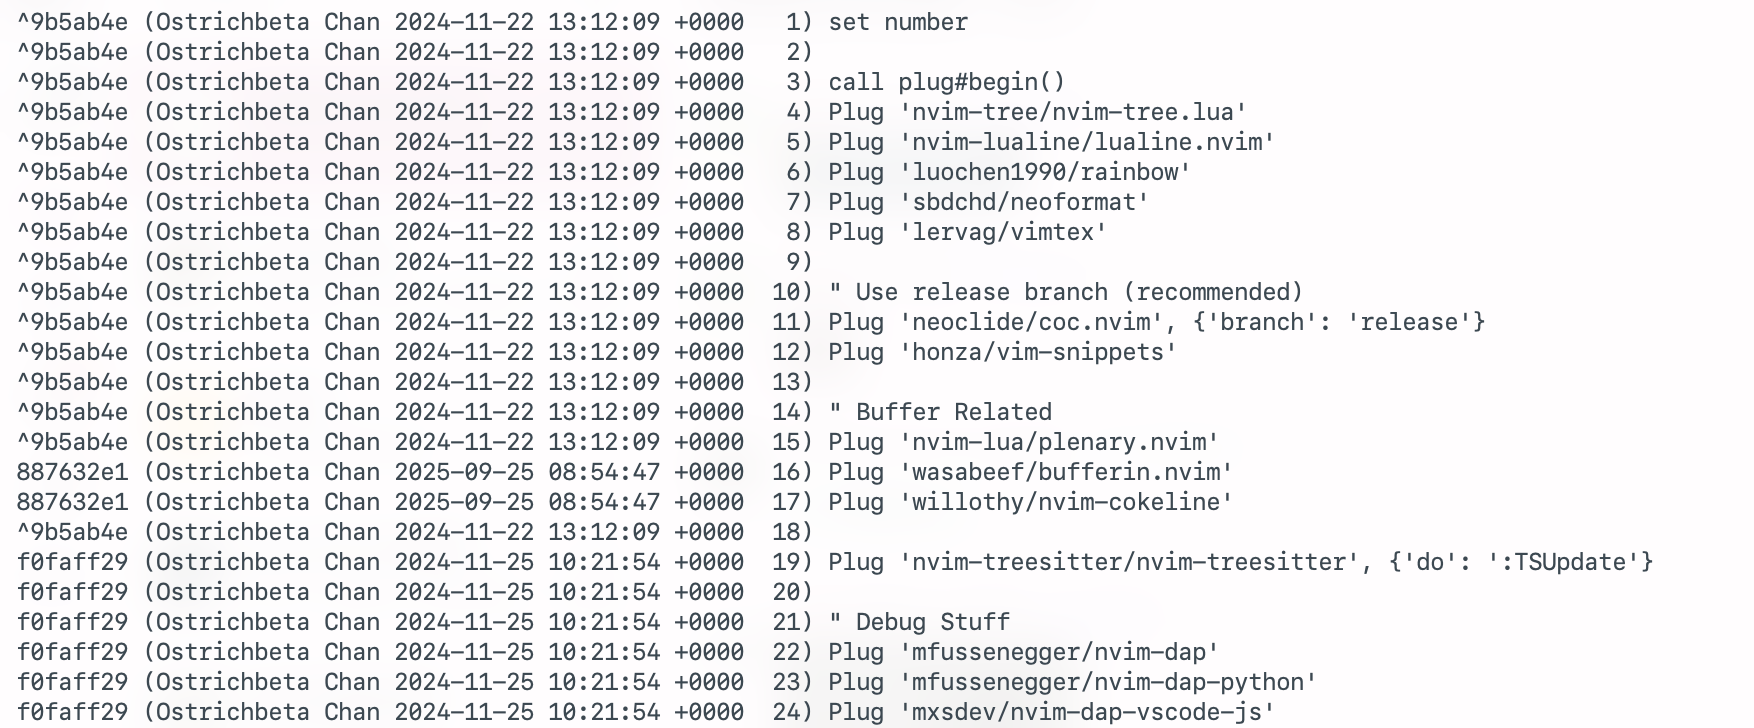
\includegraphics[width=3.6in]{./img/git-blame.png}
        \end{center}
    \end{block}
\end{frame}

\begin{frame}[fragile]{其他指令}
    \begin{block}{git revert}
        使用一個 Commit 來取消不需要的 Commit。
        \begin{lstlisting}[
          language = bash,
          numbers = none,
          linewidth = \textwidth
        ]
git revert <commit>\end{lstlisting}
        \begin{center}
            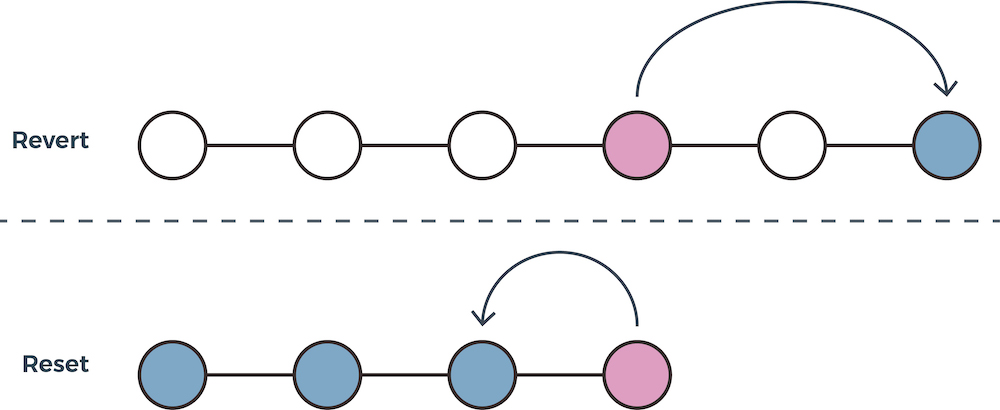
\includegraphics[width=3.3in]{./img/git-reset-vs-revert.jpg}

            \texttt{git reset} 和 \texttt{git revert} 的區別
        \end{center}
    \end{block}
\end{frame}

\begin{frame}[fragile]{其他指令}
    \begin{block}{git checkout (補充用法)}
        \texttt{git checkout} 還可以由其他分支抽出檔案。
        \begin{lstlisting}[
          language = bash,
          numbers = none,
          linewidth = \textwidth
        ]
git checkout <branch> <file> \dots # 由\texttt{branch}分支復原
git checkout [--] <file> 放棄暫存區的更改,回到暫存前狀態\end{lstlisting}
        \begin{block}{為什麼要加\texttt{--}?}
            \justify\hspace{18pt}\texttt{git checkout} 會優先匹配分支的名字。假若你有分支叫
            \texttt{c.cpp},但是同時又想復原 c.cpp 檔案,使用 \texttt{git checkout c.cpp}
            會切到 \texttt{c.cpp} 分支,唯有加上 \texttt{--} 才可以跳過分支名字的匹配直接復原檔案。
        \end{block}
    \end{block}
\end{frame}

\section{Git 遠端聯動}

\subsection{GitHub 簡介}

\begin{frame}{GitHub 是什麼}
    GitHub 是一個可以貯存、分享及與他人共同協力開發的 code 雲端託管平臺。
    使用 GitHub 存儲的倉庫可以:
    \begin{itemize}
        \item 展示或共享你的工作;
        \item 持續跟蹤和管理對於原始碼的更改;
        \item 讓他人審閱你的原始碼,給出改進的建議;
        \item 在公用專案中與他人合作,而毋須擔心你與其他專案工作者的部分會發生衝突
    \end{itemize}

    \hfill ——\ GitHub 官方文檔
\end{frame}

\begin{frame}{GitHub 是什麼}
    GitHub 上的倉庫是一個遠端倉庫,與本地倉庫聯動可以更好的將倉庫分享出去或與他人協作。
    \begin{center}
        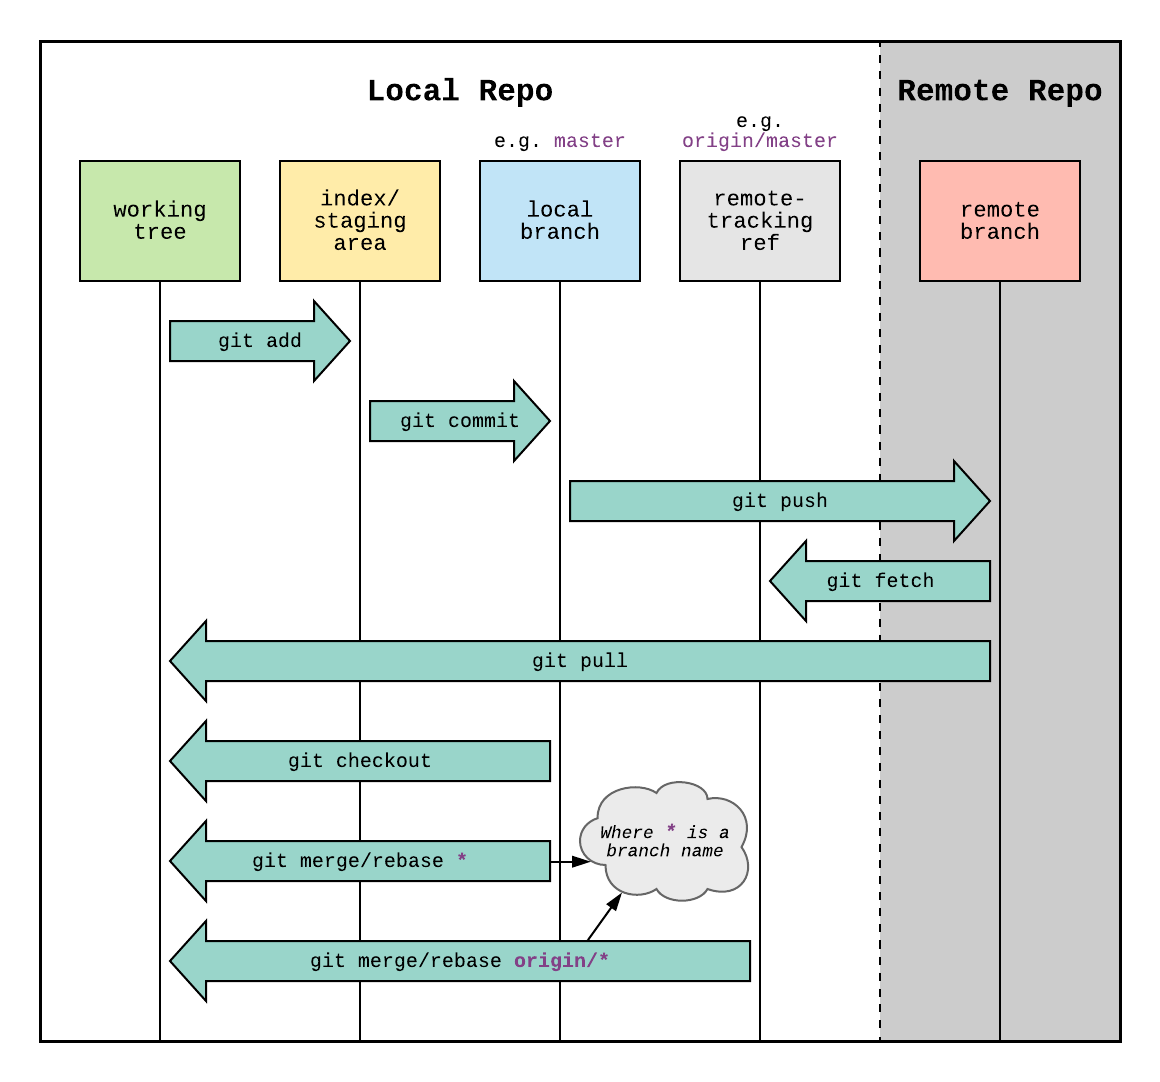
\includegraphics[width=2.7in]{./img/git-workflow.png}
    \end{center}
\end{frame}

\begin{frame}{GitHub 倉庫管理}
    \begin{block}{新增或匯入倉庫}
        按 GitHub 網頁的右上角「+」號可以選擇新增新倉庫或由其他平臺匯入已有倉庫。
        \begin{center}
            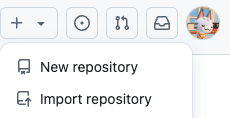
\includegraphics[width=1.5in]{./img/github-add-import-repo.png}
        \end{center}
    \end{block}
\end{frame}

\begin{frame}{GitHub 新增倉庫}
    \begin{center}
        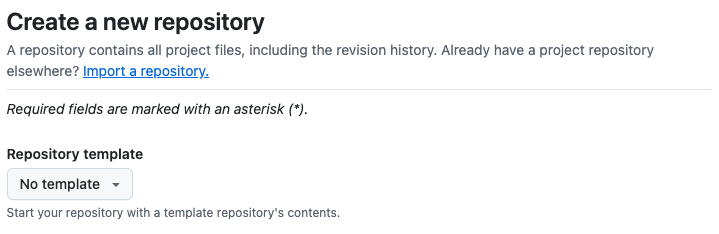
\includegraphics[width=4in]{./img/github-create-repo-0.png}
    \end{center}

    \begin{columns}
        \begin{column}{6in}
            \begin{itemize}
                \item \Emph{Repository template}\quad 根據範本新增倉庫
            \end{itemize}
        \end{column}
    \end{columns}
\end{frame}

\begin{frame}{GitHub 新增倉庫}
    \begin{center}
        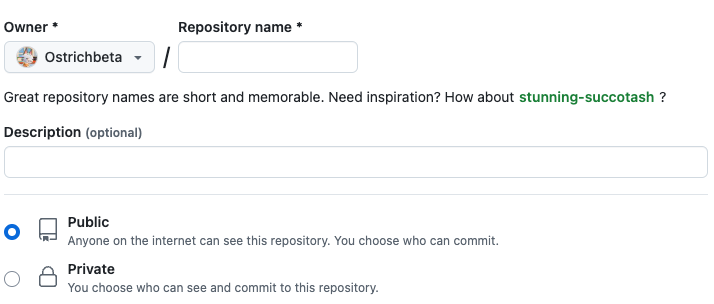
\includegraphics[width=4in]{./img/github-create-repo-1.png}

        \begin{columns}
            \begin{column}{3in}
                \begin{itemize}
                    \item \Emph{Owner}\quad 倉庫擁有者(個人或組織)
                    \item \Emph{Repo name}\quad 倉庫名字
                    \item \Emph{Description}\quad 倉庫簡介
                \end{itemize}
            \end{column}

            \begin{column}{3in}
                \begin{itemize}
                    \item \Emph{Public}\quad 公開倉庫,任何人可檢視
                    \item \Emph{Private}\quad 私有倉庫,僅自己與部分人可見
                \end{itemize}
            \end{column}
        \end{columns}
    \end{center}
\end{frame}

\begin{frame}{GitHub 新增倉庫}
    \begin{center}
        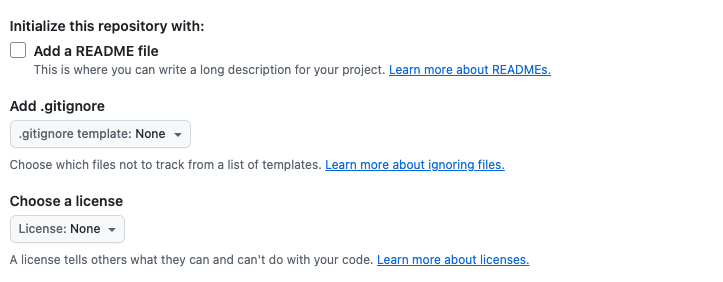
\includegraphics[width=4in]{./img/github-create-repo-2.png}
    \end{center}

    \begin{columns}
        \begin{column}{6in}
            \begin{itemize}
                \item \Emph{Add a README file}\quad 自動新增 README 檔案
                \item \Emph{Add .gitignore}\quad 按照範本新增\ .gitignore
                \item \Emph{Choose a license}\quad 選擇倉庫授權規範(Apache, BSD, GPL \dots )
            \end{itemize}
        \end{column}
    \end{columns}
\end{frame}

\begin{frame}{GitHub 新增倉庫}
    新增倉庫之後將進入倉庫頁面
    \begin{center}
        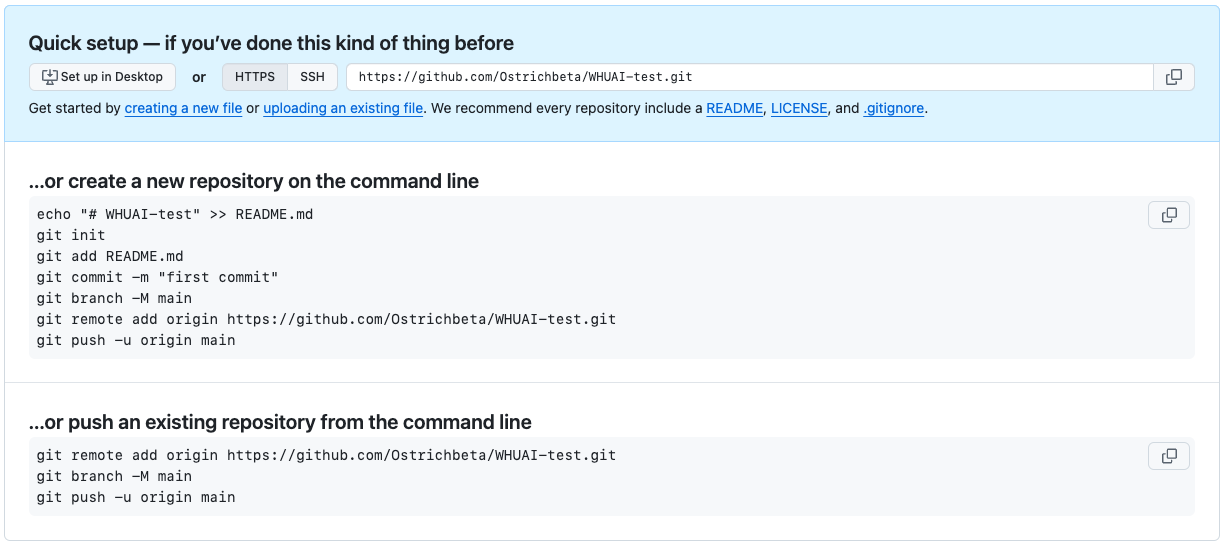
\includegraphics[width=4in]{./img/github-new-repo-tips.png}
    \end{center}
    如要刪除倉庫,在倉庫頁面 Settings - General - Danger Zone - Delete this repository
\end{frame}

\begin{frame}{GitHub 其他倉庫功能}
    \begin{center}
        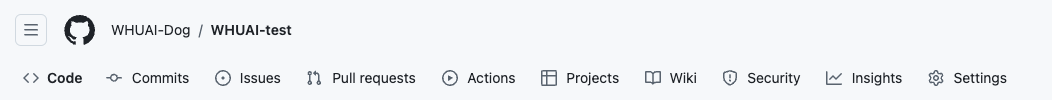
\includegraphics[width=6in]{./img/github-repo-menu.png}
    \end{center}

    \begin{itemize}
        \item \Emph{Issues}\quad 向倉庫回饋意見,反饋Bug
        \item \Emph{Pull Requests}\quad 合併自己及其他合作者提交的分支
        \item \Emph{Actions}\quad 自動化編譯及分發的流程
        \item \Emph{Projects}\quad 鏈結專案版,列出開發方向等
        \item \Emph{Wiki}\quad 可存放倉庫使用文檔
    \end{itemize}
\end{frame}

\begin{frame}{GitHub 其他倉庫功能}
    \begin{center}
        
\includegraphics[width=2.25in]{./img/github-watch-fork-star.png}
    \end{center}

    \begin{itemize}
        \item \Emph{Watch}\quad 關注倉庫,有新動向會發送電郵通知
        \item \Emph{Fork}\quad 克隆倉庫到自己的帳戶下
        \item \Emph{Star}\quad 給喜歡的項目加星標,星標更多的項目將獲更多推薦
    \end{itemize}
\end{frame}

\subsection{Git 遠端連線}

\begin{frame}{Git 遠端連線常用指令}
    涉及與遠端倉庫的聯繫時,主要會用到如下的指令:
    \begin{itemize}
        \item \texttt{git remote}
        \item \texttt{git push}
        \item \texttt{git fetch}
        \item \texttt{git pull}
        \item \texttt{git clone}
    \end{itemize}
\end{frame}

\begin{frame}[fragile]{遠端倉庫管理}
    \begin{block}{git remote}
        管理本地倉庫所鏈結的遠端倉庫。
        \begin{lstlisting}[
          language = bash,
          numbers = none,
          linewidth = \textwidth
        ]
git remote add <remote-name> <remote-url>\end{lstlisting}

        \begin{itemize}
            \item
                \texttt{\textless{}remote-name\textgreater{}}:遠端倉庫名字(可以自取),一般是 origin
            \item \texttt{\textless{}remote-url\textgreater{}}:遠端倉庫的 url
        \end{itemize}
        \pause
        一個範例如下:
        \begin{lstlisting}[
          language = bash,
          numbers = none,
          linewidth = \textwidth
        ]
git remote add origin https://github.com/Ostrichbeta/WHUAI-test.git\end{lstlisting}
    \end{block}
\end{frame}

\begin{frame}[fragile]{遠端倉庫管理}
    \begin{block}{git remote}
        \texttt{git remote} 還有其他一些指令:
        \begin{lstlisting}[
          language = bash,
          numbers = none,
          linewidth = \textwidth
        ]
git remote get-url <remote-name> # 取得遠端倉庫的 URL
git remote rm <remote-name> # 移除遠端倉庫
git remote rename <remote-name> <new-remote-name> # 重新命名遠端倉庫
git remote set-url <remote-name> <remote-url> # 變更遠端倉庫的URL
git remote show <remote-name> # 顯示遠端倉庫詳細資訊\end{lstlisting}
    \end{block}
\end{frame}

\begin{frame}[fragile]{推送至遠端倉庫}
    \begin{block}{git push}
        將本地倉庫向遠端倉庫推送,常用:
        \begin{lstlisting}[
          language = bash,
          numbers = none,
          linewidth = \textwidth
        ]
git push -u <remote-name> <branch>\end{lstlisting}
        如:
        \begin{lstlisting}[
          language = bash,
          numbers = none,
          linewidth = \textwidth
        ]
git push -u origin main\end{lstlisting}
        \begin{itemize}
            \item \texttt{-u}:設定遠端倉庫及分支,設定一次之後可以只用打 \texttt{git push} 就可推送
            \item 若目標倉庫有帳戶和密碼認證,可能還需要輸入對應的帳戶和密碼
            \item 若遠端不存在分支 \texttt{\textless{}branch\textgreater{}},會自動新增
        \end{itemize}
    \end{block}
\end{frame}

\begin{frame}{推送至遠端倉庫}
    \begin{center}
        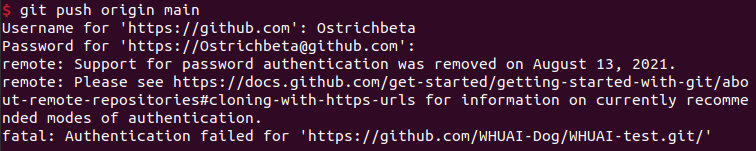
\includegraphics[width=4in]{./img/github-cannot-push.png}

        \Emph{誒,為什麼我 \texttt{push} 不上 GitHub?}
    \end{center}
    \pause
    2021 年 8 月 13 日之後,GitHub 使用者無法再使用帳戶和密碼與遠端倉庫交互,只能:
    \begin{enumerate}
        \item 生成並使用 Token,然後將 Token 用作 Git 推送時的密碼
        \item 安裝 Git Crendital Manager 並登入,使用其存儲帳戶資訊
        \item 系統生成 SSH Key 後匯入 GitHub,使用 SSH 連線
    \end{enumerate}
\end{frame}

\begin{frame}{推送至遠端倉庫}
    \begin{block}{生成Token}
        點按右上角用戶頭像 - Settings - 左側欄最下方 Developer settings - Personal access tokens

        \begin{columns}
            \begin{column}{0.3\textwidth}
                \begin{center}
                    \includegraphics[width=1.9in]{./img/github-add-key-0.png}
                \end{center}
            \end{column}

            \begin{column}{0.3\textwidth}
                \begin{center}
                    \includegraphics[width=1.9in]{./img/github-add-key-1.png}
                \end{center}
            \end{column}

            \begin{column}{0.3\textwidth}
                \begin{center}
                    \includegraphics[width=1.9in]{./img/github-add-key-2.png}
                \end{center}
            \end{column}
        \end{columns}
    \end{block}
\end{frame}

\begin{frame}{推送至遠端倉庫}
    \begin{block}{Token 種類}
        \Emph{Personal access tokens (classic)}\quad 傳統的 GitHub 使用
        Token,使用上較簡易,使用傳統的 Personal access token
        可以操作你所有有訪問許可權的倉庫。可以通過「Select scopes」可以選定 token 對於這些倉庫所具有的作用域。

        \Emph{Fine-grained tokens}\quad 比較新的 Token 格式。與傳統的 PAT 相比,對於權限的管理更加自由。
        \begin{itemize}
            \item 可以指定 Token 的適用範圍(單用戶還是組織,所有倉庫還是僅限特定倉庫)
            \item 組織管理者可以更方便下發新的 Token
            \item 與傳統 PAT 相比,Fine-grained tokens 可以設定的作用域更廣
        \end{itemize}
    \end{block}
\end{frame}

\begin{frame}{推送至遠端倉庫}
    在 Personal access tokens 介面若是選擇 Fine-grained tokens:
    \begin{enumerate}
        \item 點「Generate new token」,填寫Token名字、資源擁有者(個人或者組織)及到期日。
        \item 設定作用的倉庫範圍,選所有倉庫「All repositories」或指定的倉庫「Only select repositories」
        \item 下方的 Permissions 中設定權限,至少在「Repository
            permissions」中將「Contents」設定為「Read and write」,其他可以不設定
        \item 點按「Generate token」生成 Token,生成的 token 僅會顯示一次,請進行記錄
    \end{enumerate}
    \begin{center}
        \includegraphics[width=4.5in]{./img/github-fine-grained-token.png}
    \end{center}
\end{frame}

\begin{frame}{推送至遠端倉庫}
    在 Personal access tokens 介面若是選擇 Tokens (classic):
    \begin{enumerate}
        \item 點「Generate new token」下的「Generate new token (classic)」
        \item 設定 Token 的備註,有效期及作用域(至少勾選「repo」項)
        \item 點按下面的「Generate token」生成 Token,生成的 token 僅會顯示一次,請進行記錄
    \end{enumerate}
    \begin{center}
        \includegraphics[width=4.5in]{./img/github-pat-classic.png}
    \end{center}
\end{frame}

\begin{frame}[fragile]{推送至遠端倉庫}
    在取得對應的 Token 後,有兩種方式使用:
    \begin{itemize}
        \item 在每一次進行 \texttt{push} 操作時,於密碼處輸入所生成的 Token
        \item 在 \texttt{remote} 的 URL 中加入 Token,每一次 \texttt{push}
            操作時就不需要再輸入密碼。格式是 \texttt{https://<token>@<remote-url>},如:
    \end{itemize}
    \begin{lstlisting}[
        language = bash,
        numbers = none,
        linewidth = \textwidth
      ]
https://ghp_sMvYSxxxxx7od@github.com/WHUAI-Dog/WHUAI-test\end{lstlisting}
\end{frame}

\begin{frame}{推送至遠端倉庫}
    \begin{block}{當 \texttt{push} 發生衝突時}
        假設現在雲端比本地領先一個 commit (可能是其他開發者 \texttt{push} 的):
        \begin{center}
            \includegraphics[height=0.5in]{./img/git-push-conflict-remote.png}
            \includegraphics[height=0.5in]{./img/git-push-conflict-local.png}

            左圖:遠端,右圖:本地
        \end{center}
        如果此時本地提交了一個新的變更,並嘗試推送:
        \begin{center}
            \includegraphics[width=3in]{./img/git-push-conflict.png}
            \pause

            遠端有本地不存在的 commit,需要先拉取遠端更新才可以進行 \texttt{push}
        \end{center}
    \end{block}
\end{frame}

\begin{frame}{拉取遠端更新}
    \begin{block}{git pull}
        \justifying\hspace{17pt}拉取遠端的更新,並將其合併至本地倉庫中。無參數時 \texttt{merge}
        遠端,加 \texttt{--rebase} 時進行 \texttt{rebase} 的動作
        \begin{itemize}
            \item 如果遠端倉庫比本地新(本地沒有遠端不存在的 commit 可以直接合併)
            \item 如果遠端倉庫和本地都有對方不存在的 commit,則需要手動 \texttt{merge}
        \end{itemize}
        \begin{center}
            \includegraphics[width=2.5in]{./img/git-pull-conflict.png}
        \end{center}
    \end{block}
\end{frame}

\begin{frame}{拉取遠端更新}
    \begin{center}
        \includegraphics[width=5in]{./img/git-pull-merge.png}

        有衝突時需要手動合併
    \end{center}
\end{frame}

\begin{frame}{拉取遠端更新}
    \begin{block}{git fetch}
        僅拉取遠端倉庫的代碼,但是不進行更新。
        \begin{itemize}
            \item 「\texttt{git pull}」實際上是「\texttt{git
                fetch}」與「\texttt{git merge}」或者「\texttt{git rebase}」的組合
        \end{itemize}
        \begin{columns}
            \begin{column}{0.5\textwidth}
                \begin{center}
                    \includegraphics[height=1in]{./img/git-before-fetch.png}

                    \texttt{git fetch 之前}
                \end{center}
            \end{column}

            \begin{column}{0.5\textwidth}
                \begin{center}
                    \includegraphics[height=1in]{./img/git-after-fetch.png}

                    \texttt{git fetch 之後}
                \end{center}
            \end{column}
        \end{columns}
    \end{block}
\end{frame}

\begin{frame}{拉取遠端更新}
    \begin{block}{git fetch}
        僅拉取遠端倉庫的代碼,但是不進行更新。
        \begin{itemize}
            \item 「\texttt{git pull}」實際上是「\texttt{git
                fetch}」與「\texttt{git merge}」或者「\texttt{git rebase}」的組合
        \end{itemize}
        \begin{columns}
            \begin{column}{0.5\textwidth}
                \begin{center}
                    \includegraphics[height=1in]{./img/git-after-fetch.png}

                    \texttt{git fetch 之後}
                \end{center}
            \end{column}

            \begin{column}{0.5\textwidth}
                \begin{center}
                    \includegraphics[height=1in]{./img/git-after-fetch-merge.png}

                    \texttt{git merge 之後}
                \end{center}
            \end{column}
        \end{columns}
    \end{block}
\end{frame}

\begin{frame}[fragile]{克隆倉庫}
    \begin{block}{git clone}
        將遠端倉庫克隆至本地。
        \begin{lstlisting}[
          language = bash,
          numbers = none,
          linewidth = \textwidth
        ]
git clone <url>
git clone <url> [path]
git clone [-b <branch>] [--single-branch] [--depth n] <url> [path]\end{lstlisting}
        \begin{itemize}
            \item \texttt{path} 如果不加,預設存儲到倉庫名字相同的目錄
            \item \texttt{-b} 將本地分支切換至 \texttt{<branch>}
            \item \texttt{--single-branch} 僅克隆單一分支(有 \texttt{-b} 同步
                \texttt{<branch>},沒有預設同步主分支)
            \item \texttt{--depth} 僅同步最近 n 個 commit(預設將同步所有的 commit)
        \end{itemize}

        \texttt{--single-branch}和\texttt{--depth}指令在同步大倉庫時尤為有用。
    \end{block}
\end{frame}

\subsection{向他人的倉庫貢獻}

\begin{frame}{提交至其他人的倉庫}
    \justifying\hspace{17pt}預設情況下,每一個帳戶僅可以對自己的倉庫直接進行 \texttt{push}
    的操作,如果對於他人擁有的倉庫進行交互,則:
    \begin{itemize}
        \item 成為其他人倉庫具有直接存取(Direct access)許可權的合作者
        \item 克隆倉庫到自己帳戶,然後做出修改後提交回原始倉庫
    \end{itemize}
\end{frame}

\begin{frame}{新增倉庫合作者}
    倉庫合作者可以在項目頁面「Settings」-「Collaborators」-「Manage access」中新增倉庫具有直接存取權限的人。
    \begin{center}
        \includegraphics[width=3.5in]{./img/github-private-collaborators.png}
    \end{center}
\end{frame}

\begin{frame}{新增倉庫合作者}
    組織所擁有的倉庫可在「Settings」-「Collaborators and teams」中新增倉庫具有特定權限的人或團隊。
    \begin{center}
        \includegraphics[width=3.5in]{./img/github-private-collaborators.png}
    \end{center}
\end{frame}

\begin{frame}{克隆、更改和提交}
    將其他人所有的倉庫克隆後修改後提交,就算沒有對原始倉庫的直接訪問許可權,也可以使原倉庫獲得批准後合併自己的修改。
    \begin{enumerate}
        \item 在原倉庫使用「Fork」功能複製一份原始倉庫到自己帳戶下
        \item 對自己帳戶下的倉庫進行修改
        \item 在自己倉庫下使用「Pull requests」功能向原倉庫發起合併申請
        \item 原倉庫擁有者通過申請並處理可能的衝突之後,克隆的倉庫會合併至原始倉庫
    \end{enumerate}
\end{frame}

\begin{frame}{自動合併}
    若克隆倉庫與原始倉庫之間沒有衝突,在許可之後可以自動合併。
    \begin{center}
        \includegraphics[width=3.5in]{./img/github-pull-request-no-conflict.png}
    \end{center}
\end{frame}

\begin{frame}{自動合併}
    若克隆倉庫與原始倉庫之間沒有衝突,在許可之後可以自動合併。
    \begin{center}
        \includegraphics[width=3.5in]{./img/github-merge-pull-request-automatically.png}
    \end{center}
\end{frame}

\begin{frame}{手動合併}
    若克隆倉庫與原始倉庫之間有衝突:
    \begin{center}
        \includegraphics[width=3.5in]{./img/github-pull-request-with-conflicts.png}
    \end{center}
    \pause

    \begin{enumerate}
        \item 撤回合併申請,在克隆倉庫中 \texttt{pull} 原始倉庫解決衝突後再提交申請
        \item 由原始倉庫的維護者解決衝突
    \end{enumerate}
\end{frame}

\begin{frame}{手動合併}
    若衝突有原始倉庫的維護者解決:
    \begin{columns}
        \begin{column}{0.6\textwidth}
            \begin{center}
                \includegraphics[width=3.5in]{./img/github-merge-pull-request-manually.png}
            \end{center}
        \end{column}
        \begin{column}{0.4\textwidth}
            \begin{itemize}
                \item 在網頁中按「Resolve conflicts」手動編輯衝突部分解決
                \item 將衝突處移到本地進行處理
                    \begin{enumerate}
                        \item 原分支複製出一個合併用分支
                        \item 在複製的分支中解決衝突後合併
                        \item 在原分支中合併複製分支
                        \item 提交正常合併後的原分支
                    \end{enumerate}
            \end{itemize}
        \end{column}
    \end{columns}
\end{frame}

\begin{frame}{回退合併}
    原倉庫擁有者如果在合併之後發現原倉庫出現了重大問題,或只是單純想撤回合併,可以在合併的頁面按「Revert」將倉庫回退到合併之前的狀態。
    \begin{center}
        \includegraphics[width=4in]{./img/github-revert-pull-request.png}
    \end{center}
\end{frame}

\section{練習}
\begin{frame}{小練習}
    本倉庫有一個 zip 包的練習倉庫供練習 Git 指令。內含有 A, B, C 三個資料夾。
    \begin{enumerate}
        \item A 資料夾是一個未被 Git 管控的資料夾,初始化並完成一個 commit。
        \item B 資料夾的最新一個 commit 中,token.txt 被加入了奇怪的內容。使用 git log 查詢,並使用 git reset 或其他指令對其進行退回更新。
        \item C 資料夾中,合併 hk 分支到 main 分支,解決可能出現的合併衝突。
    \end{enumerate}

    若有不明之處,可以通過各種方式詢問搜尋引擎或者 AI 解決問題。
\end{frame}

\section{附錄}

\begin{frame}{Git 輔助資料}
    除了命令行的介面外,還可以使用一些 GUI 工具更方便 Git 的使用:
    \begin{itemize}
        \item SourceTree (Mac, Windows)
        \item GitHub Desktop (Mac, Windows)
        \item GitKraken Desktop (Mac, Linux, Windows)
        \item SmartGit (Mac, Linux, Windows)
    \end{itemize}

    可以前往
    \underline{\href{https://git-scm.com/downloads/guis}{https://git-scm.com/downloads/guis}}
    了解更多工具。

    Git
    速查表:\underline{\href{https://education.github.com/git-cheat-sheet-education.pdf}{https://education.github.com/git-cheat-sheet-education.pdf}}
\end{frame}

\begin{frame}{參考資料}
    \begin{itemize}
        \item 「為你自己學 Git」高見龍 -
            \href{https://gitbook.tw/}{\ul{https://gitbook.tw/}}
        \item
            \href{https://stackoverflow.com/questions/1274057/how-do-i-make-git-forget-about-a-file-that-was-tracked-but-is-now-in-gitignore}{\ul{https://stackoverflow.com/questions/1274057/how-do-i-make-git-forget-about-a-file-that-was-tracked-but-is-now-in-gitignore}}
        \item
            \href{https://www.reddit.com/r/git/comments/99ul9f/git_workflow_diagram_showcasing_the_role_of/}{\small
            \ul{https://www.reddit.com/r/git/comments/99ul9f/git\_workflow\_diagram\_showcasing\_the\_role\_of/}}
        \item
            \href{https://toanthien.com/blog/a-comprehensive-guide-to-git-git-merge-vs-git-rebase-and-essential-commands/}{\ul{https://toanthien.com/blog/a-comprehensive-guide-to-git-git-merge-vs-git-rebase-and-essential-commands/}}
    \end{itemize}
\end{frame}

\end{document}
